\documentclass{article}

\DeclareUnicodeCharacter{FB01}{fi}
\DeclareUnicodeCharacter{03B8}{0}

\usepackage{color}
\usepackage{graphicx}
\usepackage{amsmath}
\usepackage{bm}
\usepackage{enumerate}
\usepackage{booktabs}
\usepackage{cite}
\usepackage{geometry}
\usepackage{url}
\usepackage{float}
\usepackage{indentfirst}
\usepackage{ulem}
\usepackage[colorlinks,linkcolor=black]{hyperref}
\usepackage{multirow}
\usepackage{amssymb}
\usepackage{cite}
\usepackage{pdfpages}

\begin{document}

\vspace*{0.25cm}

\noindent\hrulefill

\thispagestyle{empty}

\begin{center}
\begin{large}
\sc{UM--SJTU Joint Institute \vspace{0.3em} \\ Physics Laboratory \\(Vp241)}
\end{large}

\hrulefill

\vspace*{5cm}
\begin{Large}
\sc{{Laboratory Report}}
\end{Large}

\vspace{2em}

\begin{large}
\sc{{Exercise 4
\vspace{0.5em}

Polarization of Light}}
\end{large}
\end{center}
\vfill

\begin{table}[h!]
\flushleft
\begin{tabular}{lll}
Name: \textbf{Kang Jiaming} \hspace*{2em}&
ID: \textbf{518021911220} \hspace*{2em}
& Group: 17\\
Name: Hong Yichen \hspace*{2em}&
ID: 518370910011\hspace*{2em}
& Group: 17\\
\\

Date: 8 Nov. 2019

\end{tabular}
\end{table}

\hfill
\newpage
\tableofcontents
\setcounter{page}{0}
\thispagestyle{empty}
\newpage

\section{Introduction\label{Ob}}

The objective of this exercise is to study the polarization of light. Specifically, Malus' law will be verified and the way how half- and quarter-wave plates work in optical systems will be explored.

\subsection{Polarization of Light}

Light in nature is electromagnetic wave. The electric field vector \textbf{E} in the electromagnetic wave is referred to as the light vector. In the plane perpendicular to the propagation direction of a light wave, the light vector may have different directions along which its magnitude oscillates. If the light vector oscillates in all possible transverse direction, the light is called \textit{natural light}. Otherwise, the light is called \textit{polarized}. The light, for which the light vector maintains a certain oscillation direction, is called \textit{linearly polarized} and the axis defining the direction is called the polarization axis. The light with the light vector direction rotating about the propagation direction, so that its endpoint traces a circle, is called \textit{circularly polarized} light. If the vector traces an ellipse, the light said to be \textit{elliptically polarized}. 

\subsection{Polarizer}

Ploarizer is a device that can produce polarized light. It polarizes the light by only allowing th light polarized in a certain direction to pass through. With such a property, it can also be used to detect and analyze the polarization state of light (it is then called an analyzer).

\subsection{Malus' Law}

A fundamental law that the polarization of light obeys is as follows.
Suppose that we have two polarizers arranged so that their planes are parallel — the left one plays the role of a polarizer, the other one is an analyzer (see Figure \ref{FigMalus}). Let the angle between their transmission directions (polarization axes) be θ. The light is incident normally on the polarizer and then continues to the analizer. The intensity of the linearly polarized light leaving the analyzer is
\begin{equation}\label{eqMalus}
I_{\text{light}} = I_{\text{light},0}\cos^2\theta,
\end{equation}
where $I_{\text{light},0}$ is the intensity of the linearly polarized light incident on the analyzer. This is the so-called Malus' law.

\begin{figure}[H]\centering
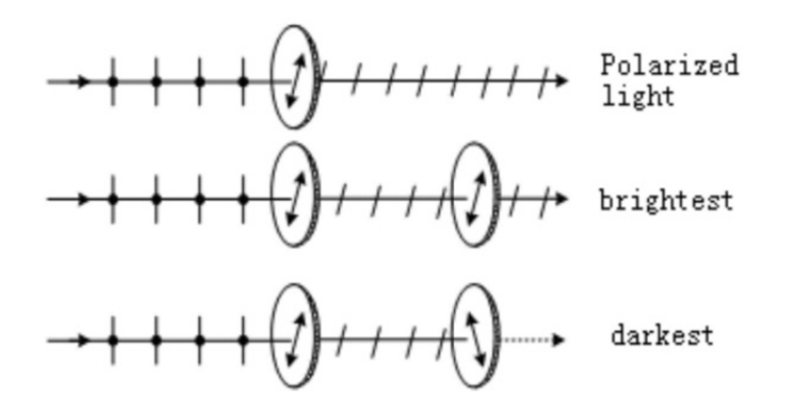
\includegraphics[scale=1.0]{polar.png}
\caption{Change in the brightness of the light depends on the mutual orientation of the polarizer and the analyzer.}\label{FigMalus}
\end{figure}

\subsection{Generation of Elliptically and Circularly Polarized Light. Half-wave and Quarter-wave Plates}
\small{\textbf{*This section is selected from [1], but the crucial points regarding this lab are highlighted here.}}

\vspace*{0.1cm}

Suppose that a linearly polarized light is incident morally on a crystal plate whose surface is parallel to its optical axis, and the angle between the polarizing axis and the optical axis of the plate is $\alpha$. Then the linearly polarized light is resolved into two waves: an e-wave with the oscillation direction parallel to the optical axis of the plate (extraordinary axis) and an o-wave whose oscillation direction is perpendicular to the optical axis (ordinary axis). They propagate in the same direction, but with different speeds. The resulting optical path difference over the thickness d of the plate is
$$\Delta = (n_\text{e} - n_\text{o})d,$$
and, consequently, the phase difference
$$\delta = \frac{2\pi}{\lambda}(n_\text{e} - n_\text{o})d,$$ 
where $\lambda$ is the wavelength, $n_\text{e}$ is the refractive index for the extraordinary axis, and $n_\text{o}$ is the refractive index for the ordinary axis. In a so-called positive crystal $\delta > 0$, whereas in a negative one $\delta < 0$.

As shown in Figure 4, when the light propagates through the crystal plate, the two components of the light vector are
\begin{align*}
E_x &= A_\text{o}\cos\omega t\\
E_y &= A_\text{e}\cos(\omega t + \delta),
\end{align*}
where $A_\text{e} = A\cos\alpha$, $A_\text{o} = A\sin\alpha$. Eliminating time from the above equations one obtains
\begin{equation}\label{eqE}
\frac{E_x^2}{A_\text{o}^2} + \frac{E_y^2}{A_\text{e}^2} - 2\frac{E_xE_y}{A_\text{o}A_\text{e}}\cos \delta = \sin^2\delta,
\end{equation}
which is the equation of an ellipse.

\begin{figure}[H]\centering
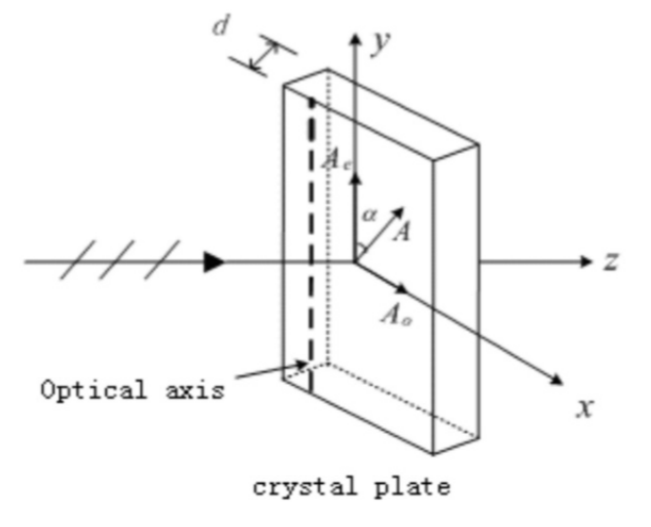
\includegraphics[scale=1.0]{crystal.png}
\caption{Linearly polarized light passing through a waveplate.}\label{FigCrystal}
\end{figure}

When the thickness of the plate changes, the optical path difference changes as well. Some cases of particular interest, are discussed below: 

\begin{enumerate}[$\blacktriangleright$]
\item If $\Delta = k\lambda$, where $k = 0,1,2,...,$ the phase difference $\delta = 0$, and Eq. (\ref{eqE}) reduces to
$$E_y = \frac{A_\text{e}}{A_\text{o}}E_x,$$
which is a linear equation. Hence the transmitted light is linearly polarized with the oscillation direction remaining unchanged. A waveplate that satisfies this condition is called a \textit{full-wave} plate. The light goes through a full-wave plate without changing its polarization state.
\item If $\Delta = (2k + 1)\lambda/2$, where $k = 0,1,2,...,$ the phase difference $\delta = \pi$, and Eq. (\ref{eqE}) simplifies to
$$E_y = -\frac{A_\text{e}}{A_\text{o}}E_x.$$  
\textbf{The transmitted light is also linearly polarized with the polarization axis rotated by the angle of $2\alpha$. A waveplate that satisfies the condition is called \textit{1/2-wave plate} or \textit{half-wave plate}. When a polarized light passes through a half-wave plate, its polarization axis gets rotated by an angle $2\alpha$.} If $\alpha = \pi/4$, then the polarization axis of the transmitted light is perpendicular to that of the incident light.
\item Finally, if $\Delta = (2k + 1)\lambda/4$, where $k = 0,1,2,...,$ the phase difference $\delta = \pm\pi/2$, and Eq. (\ref{eqE}) transforms into
$$\frac{E_x^2}{A_\text{o}^2} \pm \frac{E_y^2}{A_\text{e}^2} = 1.$$
The transmitted light is elliptically polarized with a waveplate that satisfies the above condition is called a \textit{1/4-wave plate} or a \textit{quarter-waveplate} and is an important optical element in many polarization experiments.
\end{enumerate}

If $A_\text{e} = A_\text{o} = A$, then $E^2_x +E^2_y = A^2$, and the transmitted light is circularly polarized. Since the amplitudes of the \textit{o}-wave and the \textit{e}-wave are both functions of $\alpha$, the polarization state after passing through a 1/4-wave plate will vary, depending on the angle: 

\begin{enumerate}[$\blacktriangleright$]
\item \textbf{if $\alpha = 0$, the transmitted light is linearly polarized with the polarization axis parallel to the optical axis of the 1/4-wave plate}; 
\item if $\alpha = \pi/2$, the transmitted light is linearly polarized with the polarization axis perpendicular to the optical axis of the 1/4-wave plate; 
\item \textbf{if $\alpha = \pi/4$, the transmitted light is circularly polarized}; 
\item \textbf{otherwise, the transmitted light is elliptically polarized}.
\end{enumerate}

\section{Experimental Setup}

\subsection{Apparatus}\label{Apparatus}
The experimental setup consists of a laser, a silicon photo-cell, a UT51 digital universal meter, two polarizers, a 1/2-wave plate, a 1/4-wave plate and an optical bench where the elements are placed.

The precision of the devices is shown in Table \ref{tablePresicion}.

\begin{table}[H]
\centering
\begin{tabular}{ccc}
\toprule
Instrument & Quantity & Precision\\
\midrule
Scale on the element & Angle $\theta$ & $2^\circ$\\
 Universal meter & Current $I$ & 0.001 [$\mu$A]\\
\bottomrule
\end{tabular}
\caption{Precision of the measurement instruments.}\label{tablePresicion}
\end{table}

\section{Measurement Procedure}

\subsection{Apparatus Adjustment}
\begin{enumerate}
\item Adjust the laser and the photo-cell so that the light can pass through the $\phi$ 6.0 aperture.
\item Placed the analyzer onto the optical bench, adjust its position so that the current detected is in the range 0.8 $\sim$ 1.8 $\mu$A.
\end{enumerate}

\subsection{Demonstration of Malus' Law}
\begin{enumerate}
\item Place an analyzer between the polarizer and the photo-cell. Record this value as $I_0$.
\item Adjust the angle of the analyzer until the electric current reaches 0. Set this position as $\theta = 90^\circ$.
\item Rotate the analyzer from $90^\circ$ to $0^\circ$ and record the magnitude of the current $I$ every $5^\circ$ and record the values.
\item To verify Malus' Law, plot the graph $I/I_0$ vs. $\cos^2\theta$ and perform linear fitting.
\end{enumerate}

\subsection{Linearly Polarized Light and the Half-wave Plate}
\begin{enumerate}
\item Place the 1/2-wave plate between the polarizer and the analyzer. Rotate it to make the light extinction appear again and set this position as the initial position.
\item Rotate the 1/2-wave plate for $\alpha = 10^\circ$ from the initial position and rotate the analyzer to make the light extinction appear again, record the angle of rotation $\Delta\theta$.
\item To explore the relationship, plot the graph $\Delta\theta$ vs. $\theta$.
\end{enumerate}

\subsection{Circularly and Elliptically Polarized Light and the 1/4-wave Plate}
\begin{enumerate}
\item Replace the 1/2-wave plate by the 1/4-wave plate and rotate it to make the light extinction appear and set this position as the initial position. At this point $\alpha = 0^\circ$. Then rotate the 1/4-wave plate and observe the change in the light intensity.
\item Rotate the analyzer for $360^\circ$ and record the light intensity (which is indicated by the current $I$) for every $10^\circ$ and record the data in a table.
\item Rotate the 1/4-wave plate for $20^\circ$, repeat Step 3.
\item Rotate the 1/4-wave plate for $45^\circ$, and repeat Step 3.
\item Rotate the 1/4-wave plate for $70^\circ$. Rotate the analyzer and record its position and the magnitude of the current when the light intensity reaches a maximum.
\item To find out the relation, plot the relation between the rotation angle of the analyzer and the light amplitude in polar coordinates. Normalize the amplitude by its maximum value. Mark the position recorded in Step 6 and compare it with the data recorded. 
\item To compare with the circular polarization, plot a linear fit to the data when the angle is $45^\circ$.
\end{enumerate}


\subsection*{Cautions}
\begin{enumerate}
\item Do not direct the laser beam into the eye.
\item Do not touch the surface of the polarizers or the wave plates. 
\end{enumerate}



\section{Results}

\subsection{Demonstration of Malus' Law}
The measurement data are presented in Table \ref{TableMalus}.

\begin{table}[H]\centering
\begin{tabular}{cc||cc}
\toprule
\multicolumn{2}{c}{Maximum Electric Current $I_0$} & \multicolumn{2}{c}{1.037 $\pm$ 0.001 [$\mu$A]}\\
\midrule
$\theta\,\,[^\circ] \pm 2[^\circ]$ & $I\,\,[\mu\text{A}] \pm 0.001\,\,[\mu\text{A}]$ & $\theta\,\,[^\circ] \pm 2[^\circ]$ & $I\,\,[\mu\text{A}] \pm 0.001\,\,[\mu\text{A}]$\\
\midrule
    0     & 1.037 & 50    & 0.470 \\
    5     & 1.033 & 55    & 0.373 \\
    10    & 1.014 & 60    & 0.294 \\
    15    & 0.986 & 65    & 0.206 \\
    20    & 0.947 & 70    & 0.147 \\
    25    & 0.896 & 75    & 0.085 \\
    30    & 0.822 & 80    & 0.042 \\
    35    & 0.730 & 85    & 0.015 \\
    40    & 0.643 & 90    & 0.003 \\
    45    & 0.560 &       &  \\
\bottomrule
\end{tabular}
\caption{Measurement data for Malus' law demonstration.}\label{TableMalus}
\end{table}

To find the relation between $\cos^2\theta$ and $I/I_0$, the two set of values need to be calculated first.
Take the first set of data as an example.
$$\cos^2\theta = \cos^2(0 \times \frac{\pi}{180}) = 1 \pm 0,$$
$$\frac{I}{I_0} = \frac{1.037}{1.037} = 1.0000 \pm 0.0013.$$
Perform similar calculations to each of the other sets of data and the results are shown in Table \ref{TableCI2}.

\begin{table}[H]\centering
\begin{tabular}{cccc}
\toprule
$\theta\,\,[^\circ] \pm 2\,\,[^\circ]$ & $I\,\,[\mu\text{A}] \pm 0.001\,\,[\mu\text{A}]$ & $\cos^2\theta$ & $I/I_0$\\
\midrule
    0     & 1.037 & 1     $\pm$ 0     & 1.0000 $\pm$ 0.0013 \\
    5     & 1.033 & 0.992 $\pm$ 0.006 & 0.9961 $\pm$ 0.0013 \\
    10    & 1.014 & 0.970 $\pm$ 0.012 & 0.9778 $\pm$ 0.0013 \\
    15    & 0.986 & 0.933 $\pm$ 0.017 & 0.9508 $\pm$ 0.0013 \\
    20    & 0.947 & 0.88  $\pm$ 0.02  & 0.9132 $\pm$ 0.0013 \\
    25    & 0.896 & 0.82  $\pm$ 0.03  & 0.8640 $\pm$ 0.0013 \\
    30    & 0.822 & 0.75  $\pm$ 0.03  & 0.7927 $\pm$ 0.0012 \\
    35    & 0.730 & 0.67  $\pm$ 0.03  & 0.7040 $\pm$ 0.0012 \\
    40    & 0.643 & 0.59  $\pm$ 0.03  & 0.6201 $\pm$ 0.0011 \\
    45    & 0.560 & 0.50  $\pm$ 0.03  & 0.5400 $\pm$ 0.0011 \\
    50    & 0.470 & 0.41  $\pm$ 0.03  & 0.4532 $\pm$ 0.0011 \\
    55    & 0.373 & 0.33  $\pm$ 0.03  & 0.3597 $\pm$ 0.0010 \\
    60    & 0.294 & 0.25  $\pm$ 0.03  & 0.2835 $\pm$ 0.0010 \\
    65    & 0.206 & 0.18  $\pm$ 0.03  & 0.1986 $\pm$ 0.0010 \\
    70    & 0.147 & 0.12  $\pm$ 0.02  & 0.1418 $\pm$ 0.0010 \\
    75    & 0.085 & 0.067 $\pm$ 0.017 & 0.0820 $\pm$ 0.0010 \\
    80    & 0.042 & 0.030 $\pm$ 0.012 & 0.0405 $\pm$ 0.0010 \\
    85    & 0.015 & 0.008 $\pm$ 0.006 & 0.0145 $\pm$ 0.0010 \\
    90    & 0.003 & 0     $\pm$ 0     & 0.0029 $\pm$ 0.0010 \\
\bottomrule
\end{tabular}
\caption{Result for $\cos^2\theta$ and $I/I_0$.}\label{TableCI2}
\end{table}

Then, a linear fit of the plot $I/I_0$ vs. $\theta$ are performed (Figure \ref{FigCI}). The slope of the linear fitting is 1.01 $\pm$ 0.02.

\begin{figure}[H]\centering
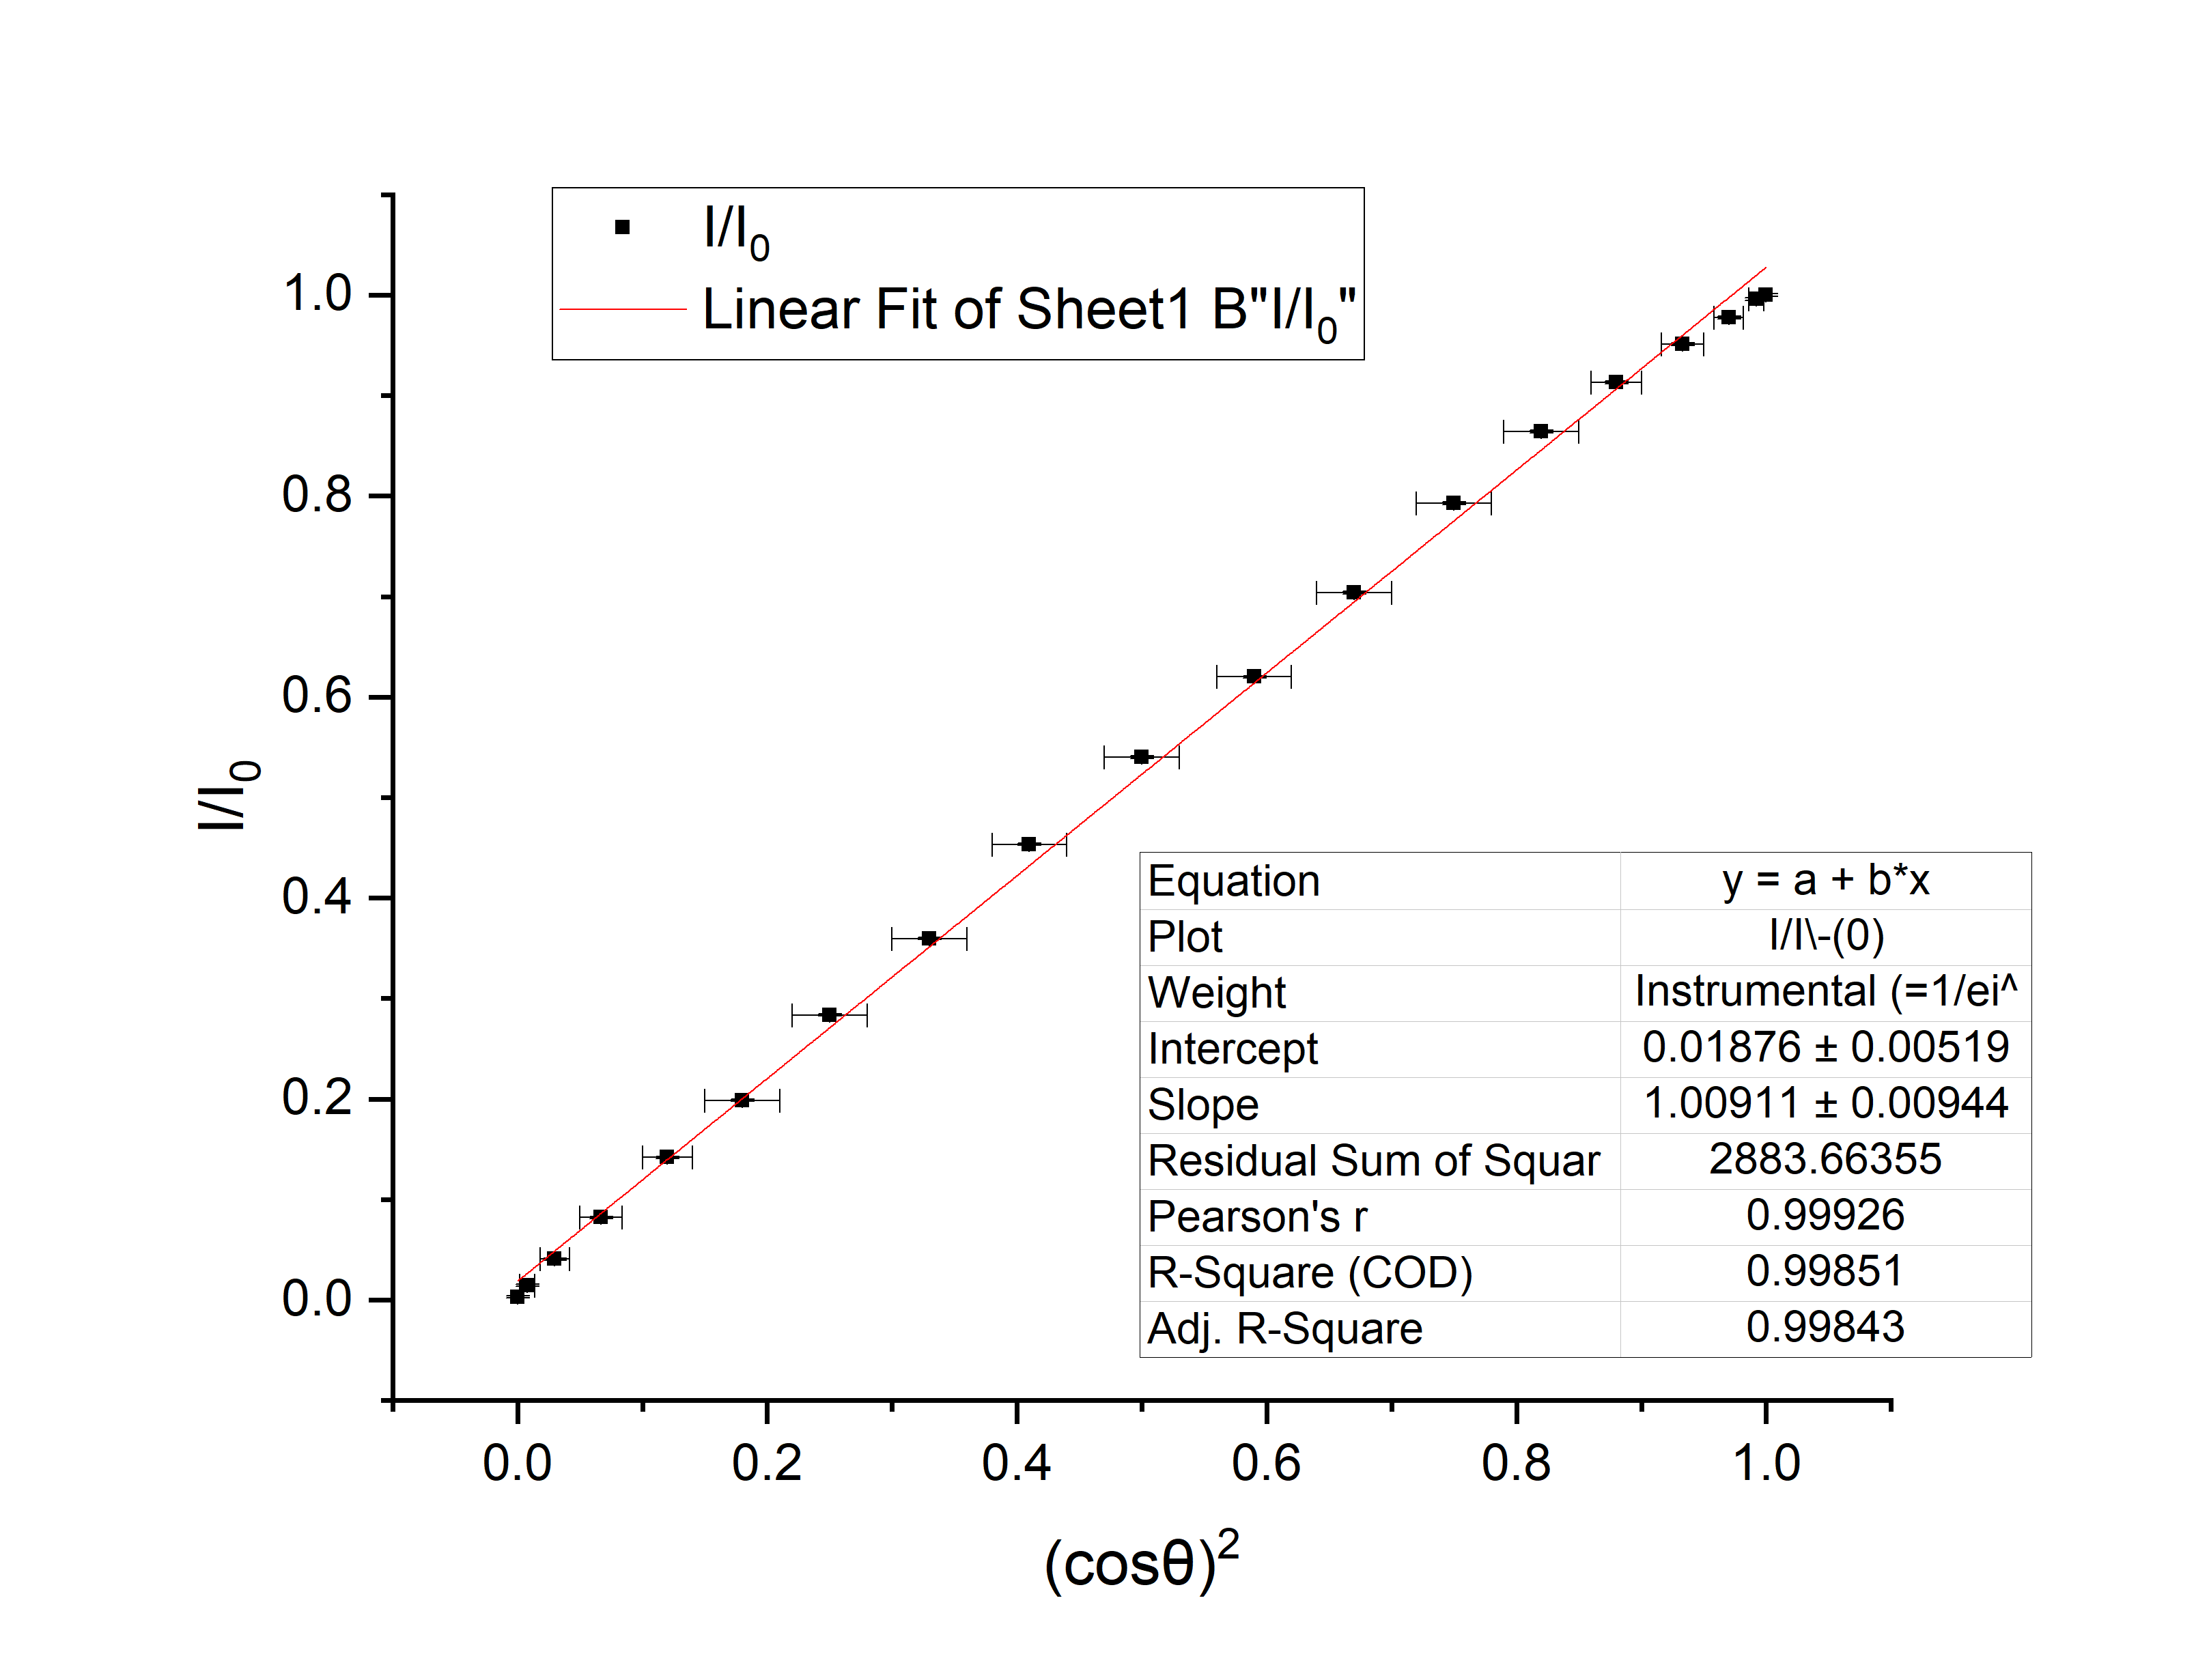
\includegraphics[scale=0.5]{1.png}
\caption{Linear fit of $I/I_0$ vs. $\cos^2\theta$ relation.}\label{FigCI}
\end{figure}


\subsection{Linearly Polarized Light and the Half-wave Plate}

The measurement data are presented in Table \ref{Table1/2}. Note that we have substracted each of the data by the initial angle in the report. 

\begin{table}[H]\centering
\begin{tabular}{cc}
\toprule
Rotation angle of the 1/2-wave plate $[^\circ] \pm 2[^\circ]$ & Rotation angle of the analyzer $[^\circ] \pm 2[^\circ]$\\
\midrule 
    initial & 0\\
    10      & 22\\
    20      & 40\\
    30      & 61\\
    40      & 82\\
    50      & 102 \\
    60      & 121 \\
    70      & 142 \\
    80      & 162 \\
    90      & 181 \\
\bottomrule
\end{tabular}
\caption{Measurement data for the 1/2-wave plate.}\label{Table1/2}
\end{table}

To find the relation between $\Delta\theta$ and $\theta$, the data are plotted in Figure \ref{Figtheta} and linear fit is performed. The slope of the linear fit is $2.01 \pm 0.02$.

\begin{figure}[H]\centering
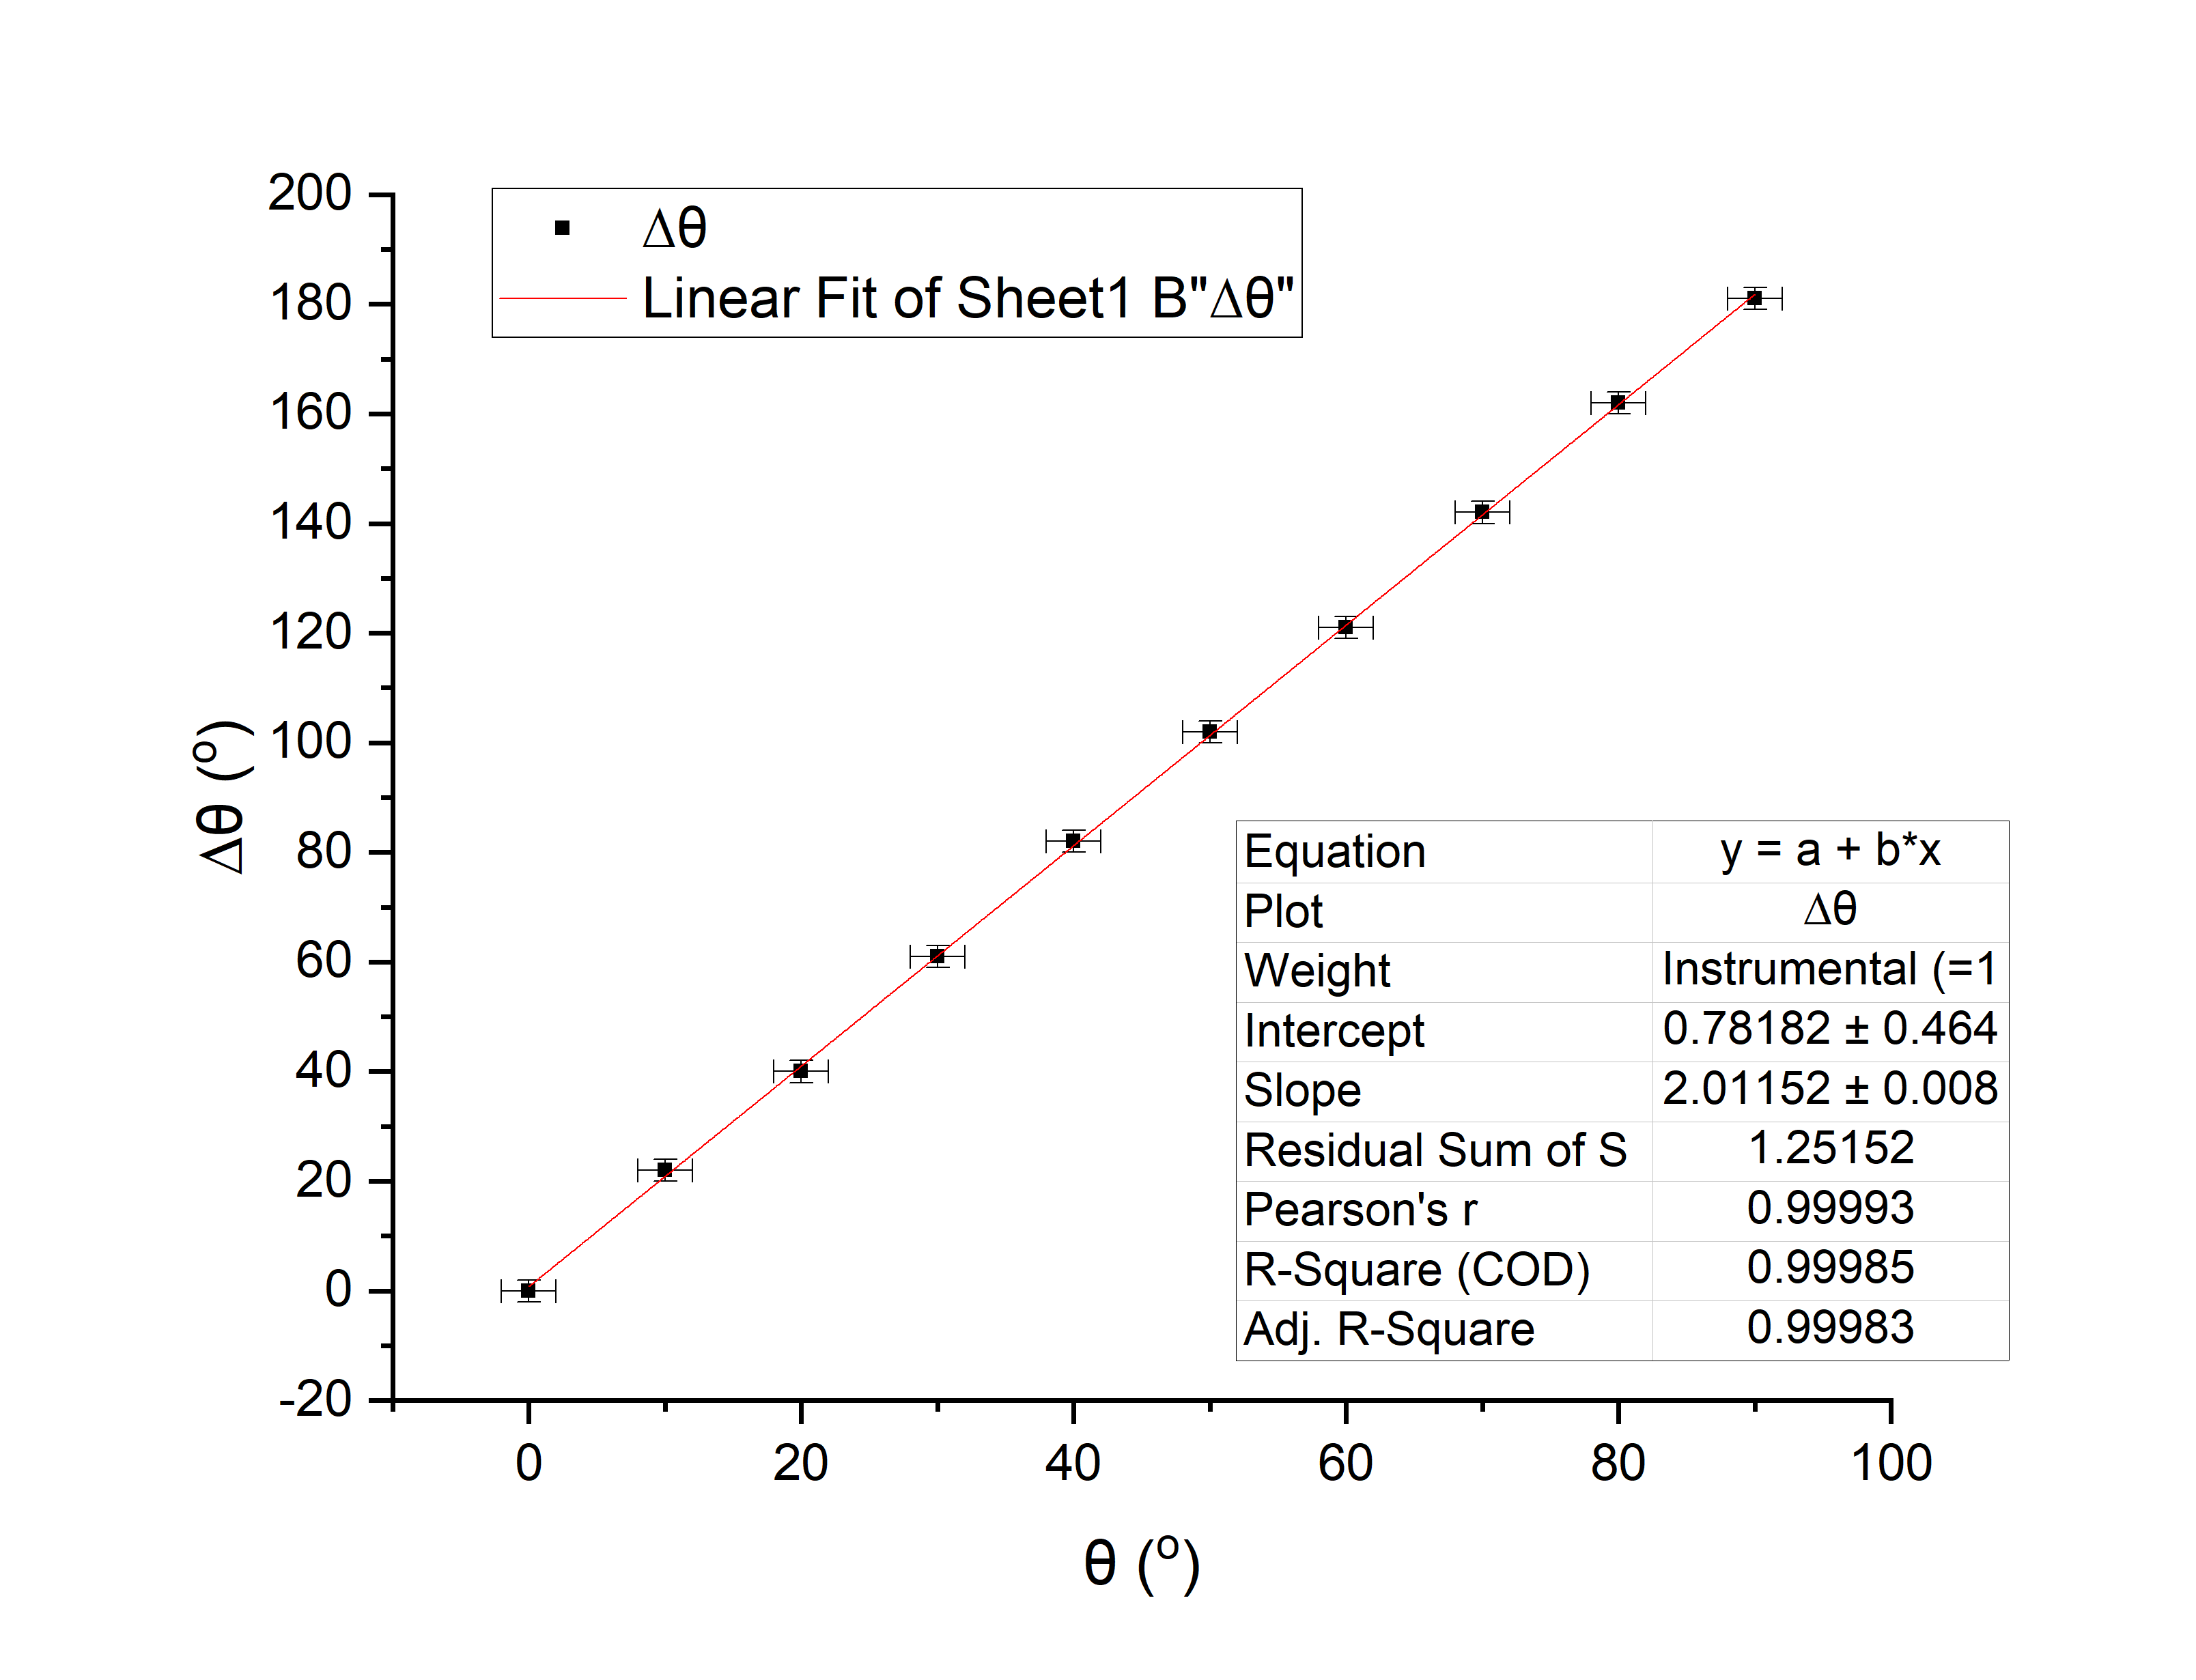
\includegraphics[scale=0.5]{2.png}
\caption{Linear fit of $\Delta\theta$ vs. $\theta$.}\label{Figtheta}
\end{figure}

Besides, in this part, when the half-wave plate rotates for 360$^\circ$, \textbf{4} times of light extinction are observed. And when the analyzer rotates 360$^\circ$, \textbf{2} times of light extinction during the analyzer rotating 360$^\circ$. It can be concluded from the above result that \textbf{the polarization axis get rotated by twice of the origin angle ($2\alpha$)} after the light passes through the 1/2-wave plate,


\subsection{Circularly and Elliptically Polarized Light and the 1/4-wave Plate}

\subsubsection{Rotation Angle: 0$^\circ$} \label{sec:0degree}

The measurement data for 0$^\circ$ rotation angle of 1/4-wave plate are presented in Table \ref{Table1/40}. Note that when filling the data sheet, 0$^\circ$ and 90 $^\circ$ are mistaken and the mistake is corrected in the report.

\begin{table}[H]\centering
\begin{tabular}{cc||cc}
\multicolumn{4}{c}{Rotation angle of 1/4-wave plate: 0$^\circ$}\\
\toprule
\multicolumn{2}{c}{Maximum Electric Current $I_0$} & \multicolumn{2}{c}{0.805 $\pm$ 0.001 [$\mu$A]}\\
\midrule
$\theta\,\,[^\circ] \pm 2[^\circ]$ & $I\,\,[\mu\text{A}] \pm 0.001\,\,[\mu\text{A}]$ & $\theta\,\,[^\circ] \pm 2[^\circ]$ & $I\,\,[\mu\text{A}] \pm 0.001\,\,[\mu\text{A}]$\\
\midrule
    0     & 0.729  & 180   & 0.805   \\
    10    & 0.716  & 190   & 0.779   \\
    20    & 0.668  & 200   & 0.706   \\
    30    & 0.570  & 210   & 0.599   \\
    40    & 0.446  & 220   & 0.470   \\
    50    & 0.316  & 230   & 0.342   \\
    60    & 0.196  & 240   & 0.210   \\
    70    & 0.093  & 250   & 0.101   \\
    80    & 0.029  & 260   & 0.031   \\
    90    & 0.003  & 270   & 0.003   \\
    100   & 0.025  & 280   & 0.023   \\
    110   & 0.091  & 290   & 0.090   \\
    120   & 0.195  & 300   & 0.195   \\
    130   & 0.317  & 310   & 0.310   \\
    140   & 0.460  & 320   & 0.421   \\
    150   & 0.596  & 330   & 0.542   \\
    160   & 0.705  & 340   & 0.649   \\
    170   & 0.779  & 350   & 0.713   \\
\bottomrule
\end{tabular}
\caption{Measurement data for the 1/4-wave plate (rotation angle 0$^\circ$).}\label{Table1/40}
\end{table}

As described in the procedure part, $\sqrt{I/I_0}$ is calculated. Take the first set of data as an example,
$$\sqrt{\frac{I}{I_0}} = \sqrt{\frac{0.729}{0.805}} = 0.9056 \pm 0.0009.$$
Perform similar calculations to each of the other sets of data and the results are presented in Table \ref{TableSqrt}.

\begin{table}[H]\centering
\begin{tabular}{cc||cc}
\toprule
$\theta\,\,[^\circ] \pm 2[^\circ]$ & $\sqrt{I/I_0}$ & $\theta\,\,[^\circ] \pm 2[^\circ]$ & $\sqrt{I/I_0}$\\
\midrule
    0     & 0.9516   $\pm$ 0.0009  & 180   & 1.0000   $\pm$ 0.0009  \\
    10    & 0.9431   $\pm$ 0.0009  & 190   & 0.9837   $\pm$ 0.0009  \\
    20    & 0.9109   $\pm$ 0.0009  & 200   & 0.9365   $\pm$ 0.0009  \\
    30    & 0.8415   $\pm$ 0.0009  & 210   & 0.8626   $\pm$ 0.0009  \\
    40    & 0.7443   $\pm$ 0.0010  & 220   & 0.7641   $\pm$ 0.0009  \\
    50    & 0.6265   $\pm$ 0.0011  & 230   & 0.6518   $\pm$ 0.0010  \\
    60    & 0.4934   $\pm$ 0.0013  & 240   & 0.5108   $\pm$ 0.0013  \\
    70    & 0.3399   $\pm$ 0.0018  & 250   & 0.3542   $\pm$ 0.0018  \\
    80    & 0.190    $\pm$ 0.003   & 260   & 0.196    $\pm$ 0.003   \\
    90    & 0.061    $\pm$ 0.010   & 270   & 0.061    $\pm$ 0.010   \\
    100   & 0.176    $\pm$ 0.004   & 280   & 0.169    $\pm$ 0.004   \\
    110   & 0.3362   $\pm$ 0.0019  & 290   & 0.3344   $\pm$ 0.0019  \\
    120   & 0.4922   $\pm$ 0.0013  & 300   & 0.4922   $\pm$ 0.0013  \\
    130   & 0.6275   $\pm$ 0.0011  & 310   & 0.6206   $\pm$ 0.0011  \\
    140   & 0.7559   $\pm$ 0.0009  & 320   & 0.7232   $\pm$ 0.0010  \\
    150   & 0.8604   $\pm$ 0.0009  & 330   & 0.8205   $\pm$ 0.0009  \\
    160   & 0.9358   $\pm$ 0.0009  & 340   & 0.8979   $\pm$ 0.0009  \\
    170   & 0.9837   $\pm$ 0.0009  & 350   & 0.9411   $\pm$ 0.0009  \\
\bottomrule
\end{tabular}
\caption{Results for $\sqrt{I/I_0}$ when rotation angle is 0$^\circ$.}\label{TableSqrt}
\end{table}

Then the relationship of $\sqrt{I/I_0}$ and $\theta$ are plotted in polar coordinate (Figure \ref{Fig0}).

\begin{figure}[H]\centering
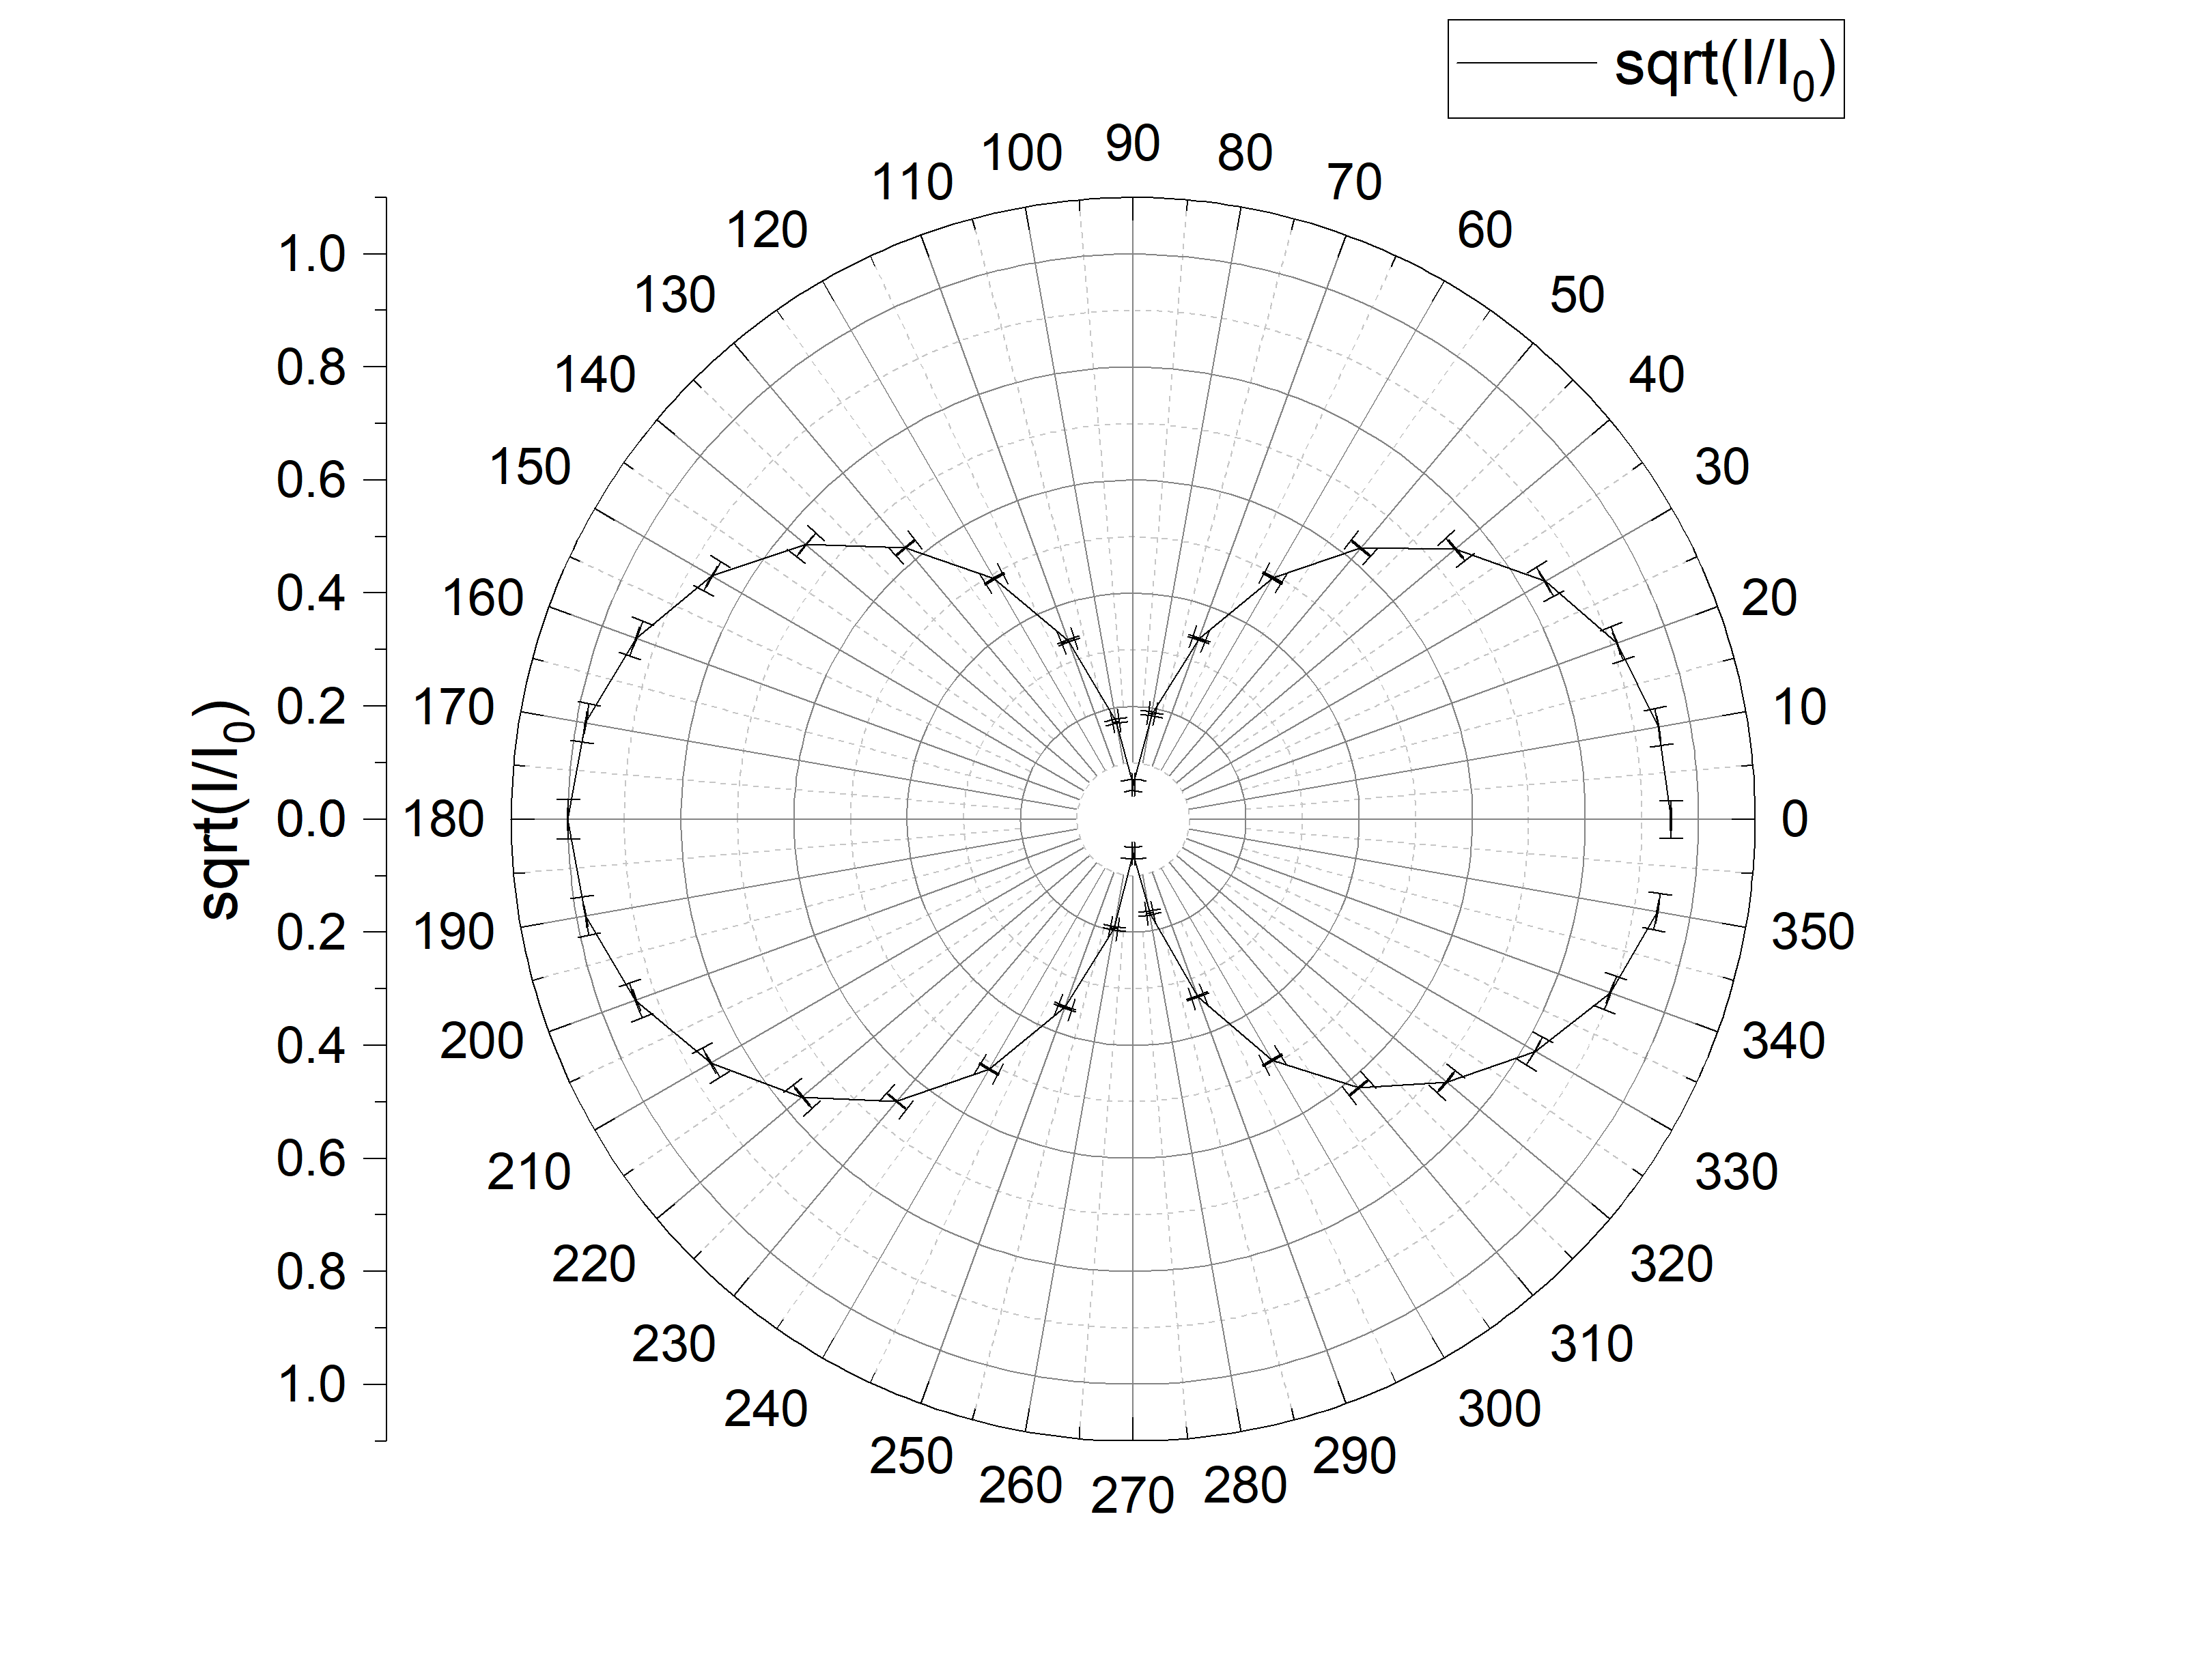
\includegraphics[scale=0.45]{3.png}
\caption{$\sqrt{I/I_0}$ vs. $\theta$ relation in polar coordinate when rotation angle is 0$^\circ$.}\label{Fig0}
\end{figure}


\subsubsection{Rotation Angle: 20$^\circ$}

The measurement data for 20$^\circ$ rotation angle of 1/4-wave plate are shown in Table \ref{Table1/420}.  Note that when filling the data sheet, 0$^\circ$ and 90 $^\circ$ are mistaken and the mistake is corrected in the report.

\begin{table}[H]\centering
\begin{tabular}{cc||cc}
\multicolumn{4}{c}{Rotation angle of 1/4-wave plate: 20$^\circ$}\\
\toprule
\multicolumn{2}{c}{Maximum Electric Current $I_0$} & \multicolumn{2}{c}{0.707 $\pm$ 0.001 [$\mu$A]}\\
\midrule
$\theta\,\,[^\circ] \pm 2[^\circ]$ & $I\,\,[\mu\text{A}] \pm 0.001\,\,[\mu\text{A}]$ & $\theta\,\,[^\circ] \pm 2[^\circ]$ & $I\,\,[\mu\text{A}] \pm 0.001\,\,[\mu\text{A}]$\\
\midrule
    0     & 0.589 & 180   & 0.641 \\
    10    & 0.646 & 190   & 0.693 \\
    20    & 0.671 & 200   & 0.707 \\
    30    & 0.662 & 210   & 0.690 \\
    40    & 0.612 & 220   & 0.644 \\
    50    & 0.534 & 230   & 0.567 \\
    60    & 0.453 & 240   & 0.470 \\
    70    & 0.356 & 250   & 0.363 \\
    80    & 0.261 & 260   & 0.263 \\
    90    & 0.179 & 270   & 0.184 \\
    100   & 0.123 & 280   & 0.127 \\
    110   & 0.102 & 290   & 0.104 \\
    120   & 0.116 & 300   & 0.115 \\
    130   & 0.164 & 310   & 0.159 \\
    140   & 0.240 & 320   & 0.224 \\
    150   & 0.345 & 330   & 0.318 \\
    160   & 0.450 & 340   & 0.420 \\
    170   & 0.550 & 350   & 0.513 \\
\bottomrule
\end{tabular}
\caption{Measurement data for the 1/4-wave plate (rotation angle 20$^\circ$).}\label{Table1/420}
\end{table}

Similar to the previous section, $\sqrt{I/I_0}$ is calculated and the results are presented in Table \ref{TableSqrt20} (For sample calculation please refer to section \ref{sec:0degree}, which will not be repeated here).

\begin{table}[H]\centering
\begin{tabular}{cc||cc}
\toprule
$\theta\,\,[^\circ] \pm 2[^\circ]$ & $\sqrt{I/I_0}$ & $\theta\,\,[^\circ] \pm 2[^\circ]$ & $\sqrt{I/I_0}$\\
\midrule
    0     & 0.9127   $\pm$ 0.0010  & 180   & 0.9522  $\pm$ 0.0010  \\
    10    & 0.9559   $\pm$ 0.0010  & 190   & 0.9900  $\pm$ 0.0010  \\
    20    & 0.9742   $\pm$ 0.0010  & 200   & 1.0000  $\pm$ 0.0010  \\
    30    & 0.9677   $\pm$ 0.0010  & 210   & 0.9879  $\pm$ 0.0010  \\
    40    & 0.9304   $\pm$ 0.0010  & 220   & 0.9544  $\pm$ 0.0010  \\
    50    & 0.8691   $\pm$ 0.0010  & 230   & 0.8955  $\pm$ 0.0010  \\
    60    & 0.8005   $\pm$ 0.0010  & 240   & 0.8153  $\pm$ 0.0010  \\
    70    & 0.7096   $\pm$ 0.0011  & 250   & 0.7165  $\pm$ 0.0011  \\
    80    & 0.6076   $\pm$ 0.0012  & 260   & 0.6099  $\pm$ 0.0012  \\
    90    & 0.5032   $\pm$ 0.0014  & 270   & 0.5102  $\pm$ 0.0014  \\
    100   & 0.4171   $\pm$ 0.0017  & 280   & 0.4238  $\pm$ 0.0017  \\
    110   & 0.3798   $\pm$ 0.0019  & 290   & 0.3835  $\pm$ 0.0019  \\
    120   & 0.4051   $\pm$ 0.0018  & 300   & 0.4033  $\pm$ 0.0018  \\
    130   & 0.4816   $\pm$ 0.0015  & 310   & 0.4742  $\pm$ 0.0015  \\
    140   & 0.5826   $\pm$ 0.0013  & 320   & 0.5629  $\pm$ 0.0013  \\
    150   & 0.6986   $\pm$ 0.0011  & 330   & 0.6707  $\pm$ 0.0012  \\
    160   & 0.7978   $\pm$ 0.0011  & 340   & 0.7708  $\pm$ 0.0011  \\
    170   & 0.8820   $\pm$ 0.0010  & 350   & 0.8518  $\pm$ 0.0010  \\
\bottomrule
\end{tabular}
\caption{Results for $\sqrt{I/I_0}$ when rotation angle is 20$^\circ$.}\label{TableSqrt20}
\end{table}

Then the relationship of $\sqrt{I/I_0}$ and $\theta$ are plotted in polar coordinate (Figure \ref{Fig20}).

\begin{figure}[H]\centering
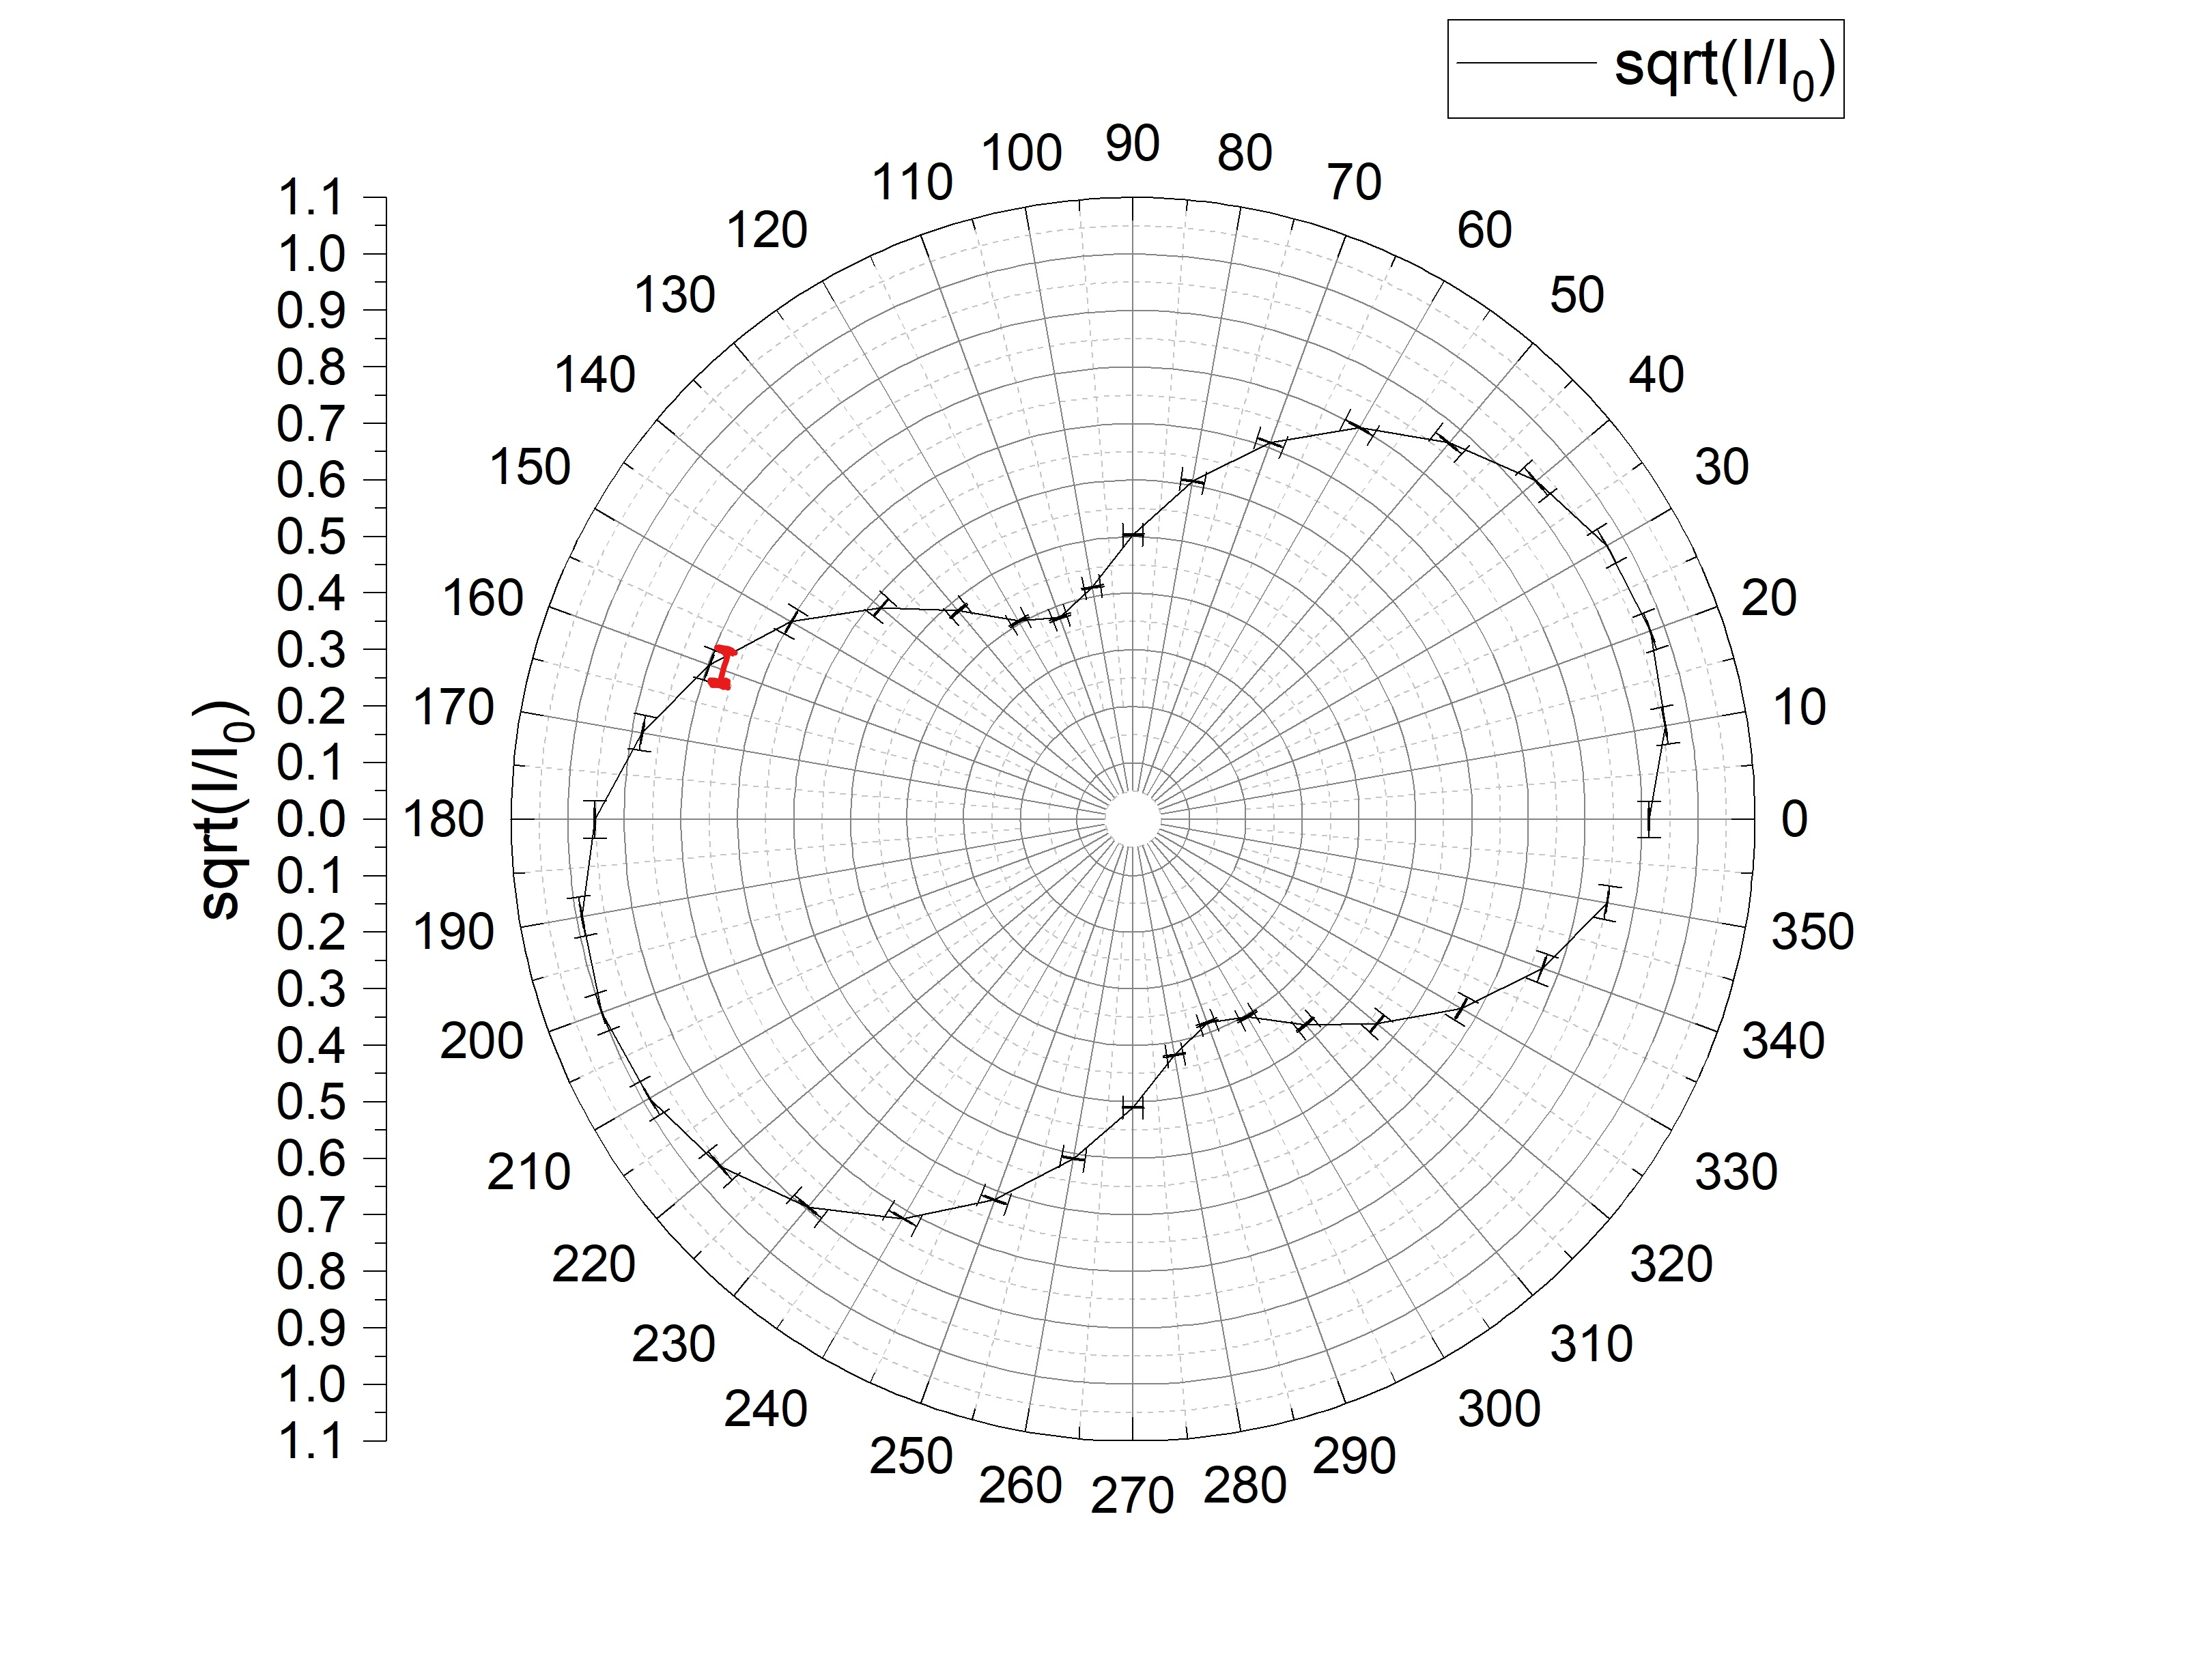
\includegraphics[scale=0.12]{4.jpg}
\caption{$\sqrt{I/I_0}$ vs. $\theta$ relation in polar coordinate when rotation angle is 20$^\circ$, together with the maximum point of rotation angle 70$^\circ$(marked in red).}\label{Fig20}
\end{figure}


\subsubsection{Rotation Angle: 45$^\circ$}

The measurement data for 45$^\circ$ rotation angle of 1/4-wave plate are shown in Table \ref{Table1/445}.  Note that when filling the data sheet, 0$^\circ$ and 90$^\circ$ are mistaken and the mistake is corrected in the report.

\begin{table}[H]\centering
\begin{tabular}{cc||cc}
\multicolumn{4}{c}{Rotation angle of 1/4-wave plate: 45$^\circ$}\\
\toprule
\multicolumn{2}{c}{Maximum Electric Current $I_0$} & \multicolumn{2}{c}{0.395 $\pm$ 0.001 [$\mu$A]}\\
\midrule
$\theta\,\,[^\circ] \pm 2[^\circ]$ & $I\,\,[\mu\text{A}] \pm 0.001\,\,[\mu\text{A}]$ & $\theta\,\,[^\circ] \pm 2[^\circ]$ & $I\,\,[\mu\text{A}] \pm 0.001\,\,[\mu\text{A}]$\\
\midrule
    0     & 0.359  & 180   & 0.392  \\
    10    & 0.360  & 190   & 0.387  \\
    20    & 0.356  & 200   & 0.378  \\
    30    & 0.354  & 210   & 0.370  \\
    40    & 0.351  & 220   & 0.368  \\
    50    & 0.348  & 230   & 0.365  \\
    60    & 0.354  & 240   & 0.363  \\
    70    & 0.361  & 250   & 0.365  \\
    80    & 0.364  & 260   & 0.369  \\
    90    & 0.371  & 270   & 0.375  \\
    100   & 0.375  & 280   & 0.386  \\
    110   & 0.381  & 290   & 0.392  \\
    120   & 0.385  & 300   & 0.389  \\
    130   & 0.390  & 310   & 0.378  \\
    140   & 0.393  & 320   & 0.366  \\
    150   & 0.395  & 330   & 0.365  \\
    160   & 0.393  & 340   & 0.369  \\
    170   & 0.395  & 350   & 0.364  \\
\bottomrule
\end{tabular}
\caption{Measurement data for the 1/4-wave plate (rotation angle 45$^\circ$).}\label{Table1/445}
\end{table}

Similar to the previous section, $\sqrt{I/I_0}$ is calculated and the results are presented in Table \ref{TableSqrt45} (For sample calculation please refer to section \ref{sec:0degree}, which will not be repeated here).

\begin{table}[H]\centering
\begin{tabular}{cc||cc}
\toprule
$\theta\,\,[^\circ] \pm 2[^\circ]$ & $\sqrt{I/I_0}$ & $\theta\,\,[^\circ] \pm 2[^\circ]$ & $\sqrt{I/I_0}$\\
\midrule
    0     & 0.9533  $\pm$ 0.0018  & 180   & 0.9962  $\pm$ 0.0018 \\
    10    & 0.9547  $\pm$ 0.0018  & 190   & 0.9898  $\pm$ 0.0018 \\
    20    & 0.9494  $\pm$ 0.0018  & 200   & 0.9782  $\pm$ 0.0018 \\
    30    & 0.9467  $\pm$ 0.0018  & 210   & 0.9678  $\pm$ 0.0018 \\
    40    & 0.9427  $\pm$ 0.0018  & 220   & 0.9652  $\pm$ 0.0018 \\
    50    & 0.9386  $\pm$ 0.0018  & 230   & 0.9613  $\pm$ 0.0018 \\
    60    & 0.9467  $\pm$ 0.0018  & 240   & 0.9586  $\pm$ 0.0018 \\
    70    & 0.9560  $\pm$ 0.0018  & 250   & 0.9613  $\pm$ 0.0018 \\
    80    & 0.9600  $\pm$ 0.0018  & 260   & 0.9665  $\pm$ 0.0018 \\
    90    & 0.9691  $\pm$ 0.0018  & 270   & 0.9744  $\pm$ 0.0018 \\
    100   & 0.9744  $\pm$ 0.0018  & 280   & 0.9885  $\pm$ 0.0018 \\
    110   & 0.9821  $\pm$ 0.0018  & 290   & 0.9962  $\pm$ 0.0018 \\
    120   & 0.9873  $\pm$ 0.0018  & 300   & 0.9924  $\pm$ 0.0018 \\
    130   & 0.9937  $\pm$ 0.0018  & 310   & 0.9782  $\pm$ 0.0018 \\
    140   & 0.9975  $\pm$ 0.0018  & 320   & 0.9626  $\pm$ 0.0018 \\
    150   & 1.0000  $\pm$ 0.0018  & 330   & 0.9613  $\pm$ 0.0018 \\
    160   & 0.9975  $\pm$ 0.0018  & 340   & 0.9665  $\pm$ 0.0018 \\
    170   & 1.0000  $\pm$ 0.0018  & 350   & 0.9600  $\pm$ 0.0018 \\
\bottomrule
\end{tabular}
\caption{Results for $\sqrt{I/I_0}$ when rotation angle is 45$^\circ$.}\label{TableSqrt45}
\end{table}

Then the relationship of $\sqrt{I/I_0}$ and $\theta$ are plotted in polar coordinate (Figure \ref{Fig45}).

\begin{figure}[H]\centering
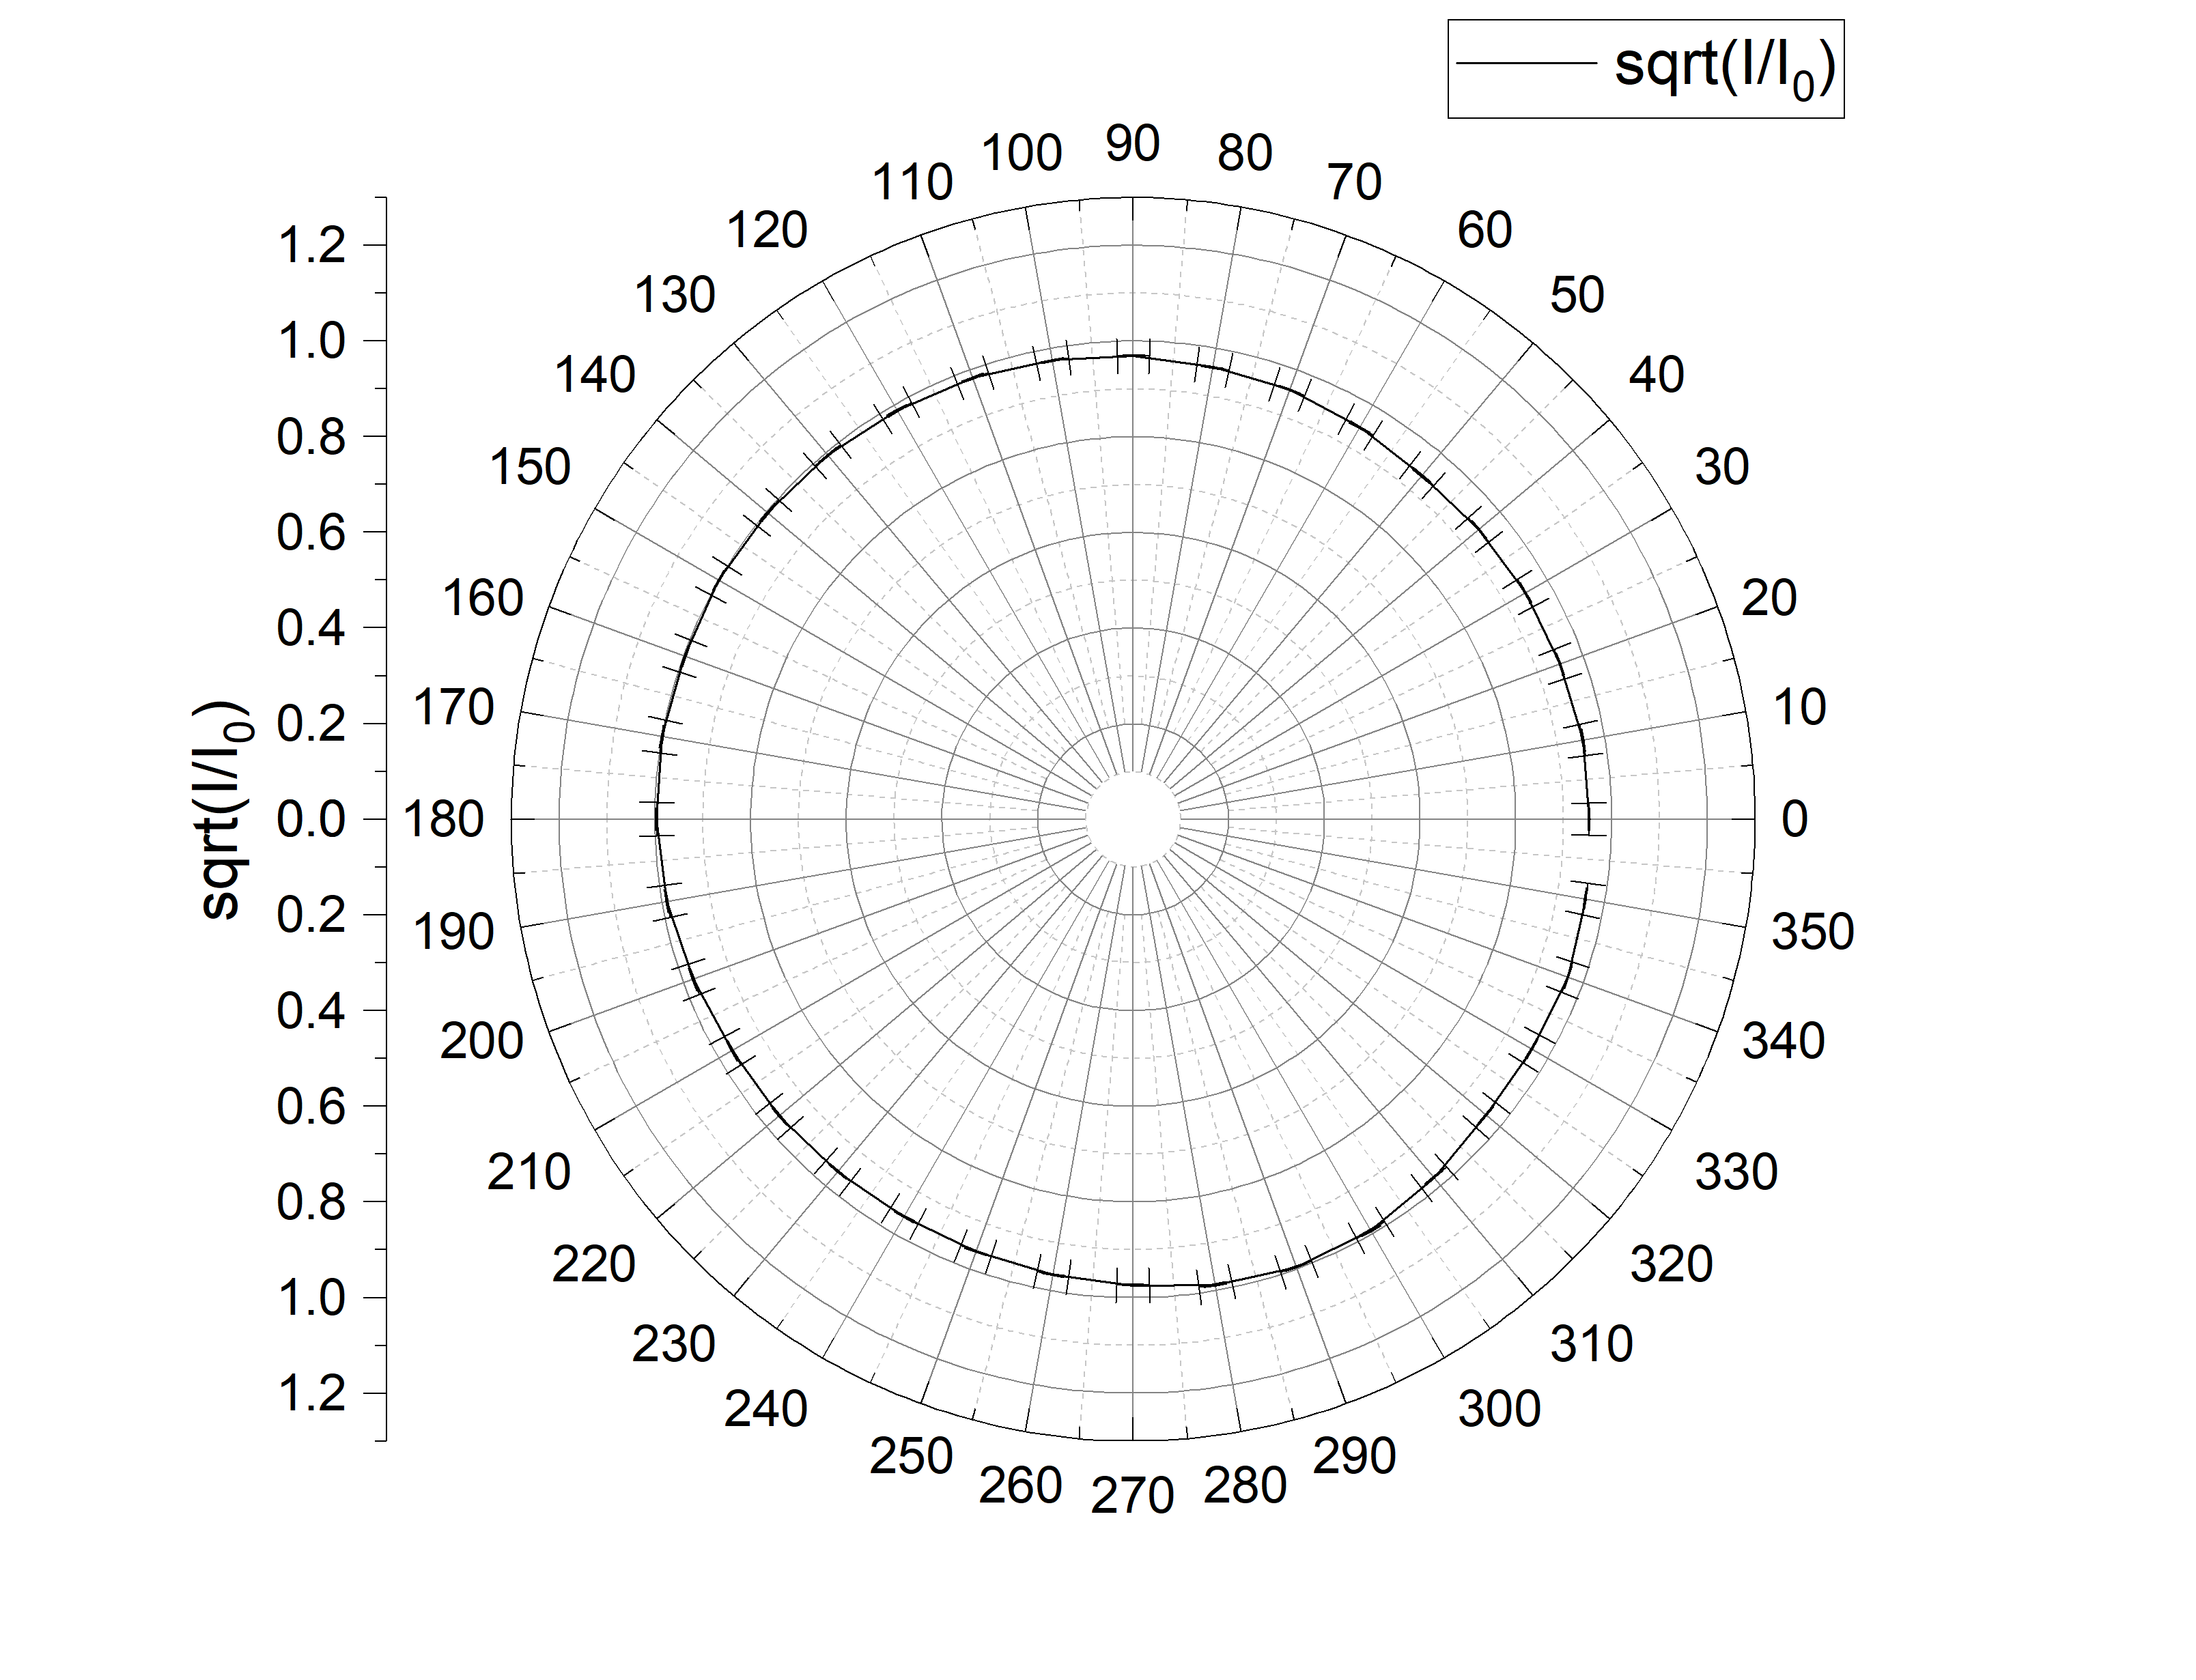
\includegraphics[scale=0.45]{5.png}
\caption{$\sqrt{I/I_0}$ vs. $\theta$ relation in polar coordinate when rotation angle is 45$^\circ$.}\label{Fig45}
\end{figure}

To compare the result with circular polarization, as described in the procedure part, the data is also plotted in Cartesian coordinate and linear fit is performed (Figure \ref{Fig45l}). The slope of the linear fitting is $6 \times 10^{-5} \pm 6 \times 10^{-5}$.

\begin{figure}[H]\centering
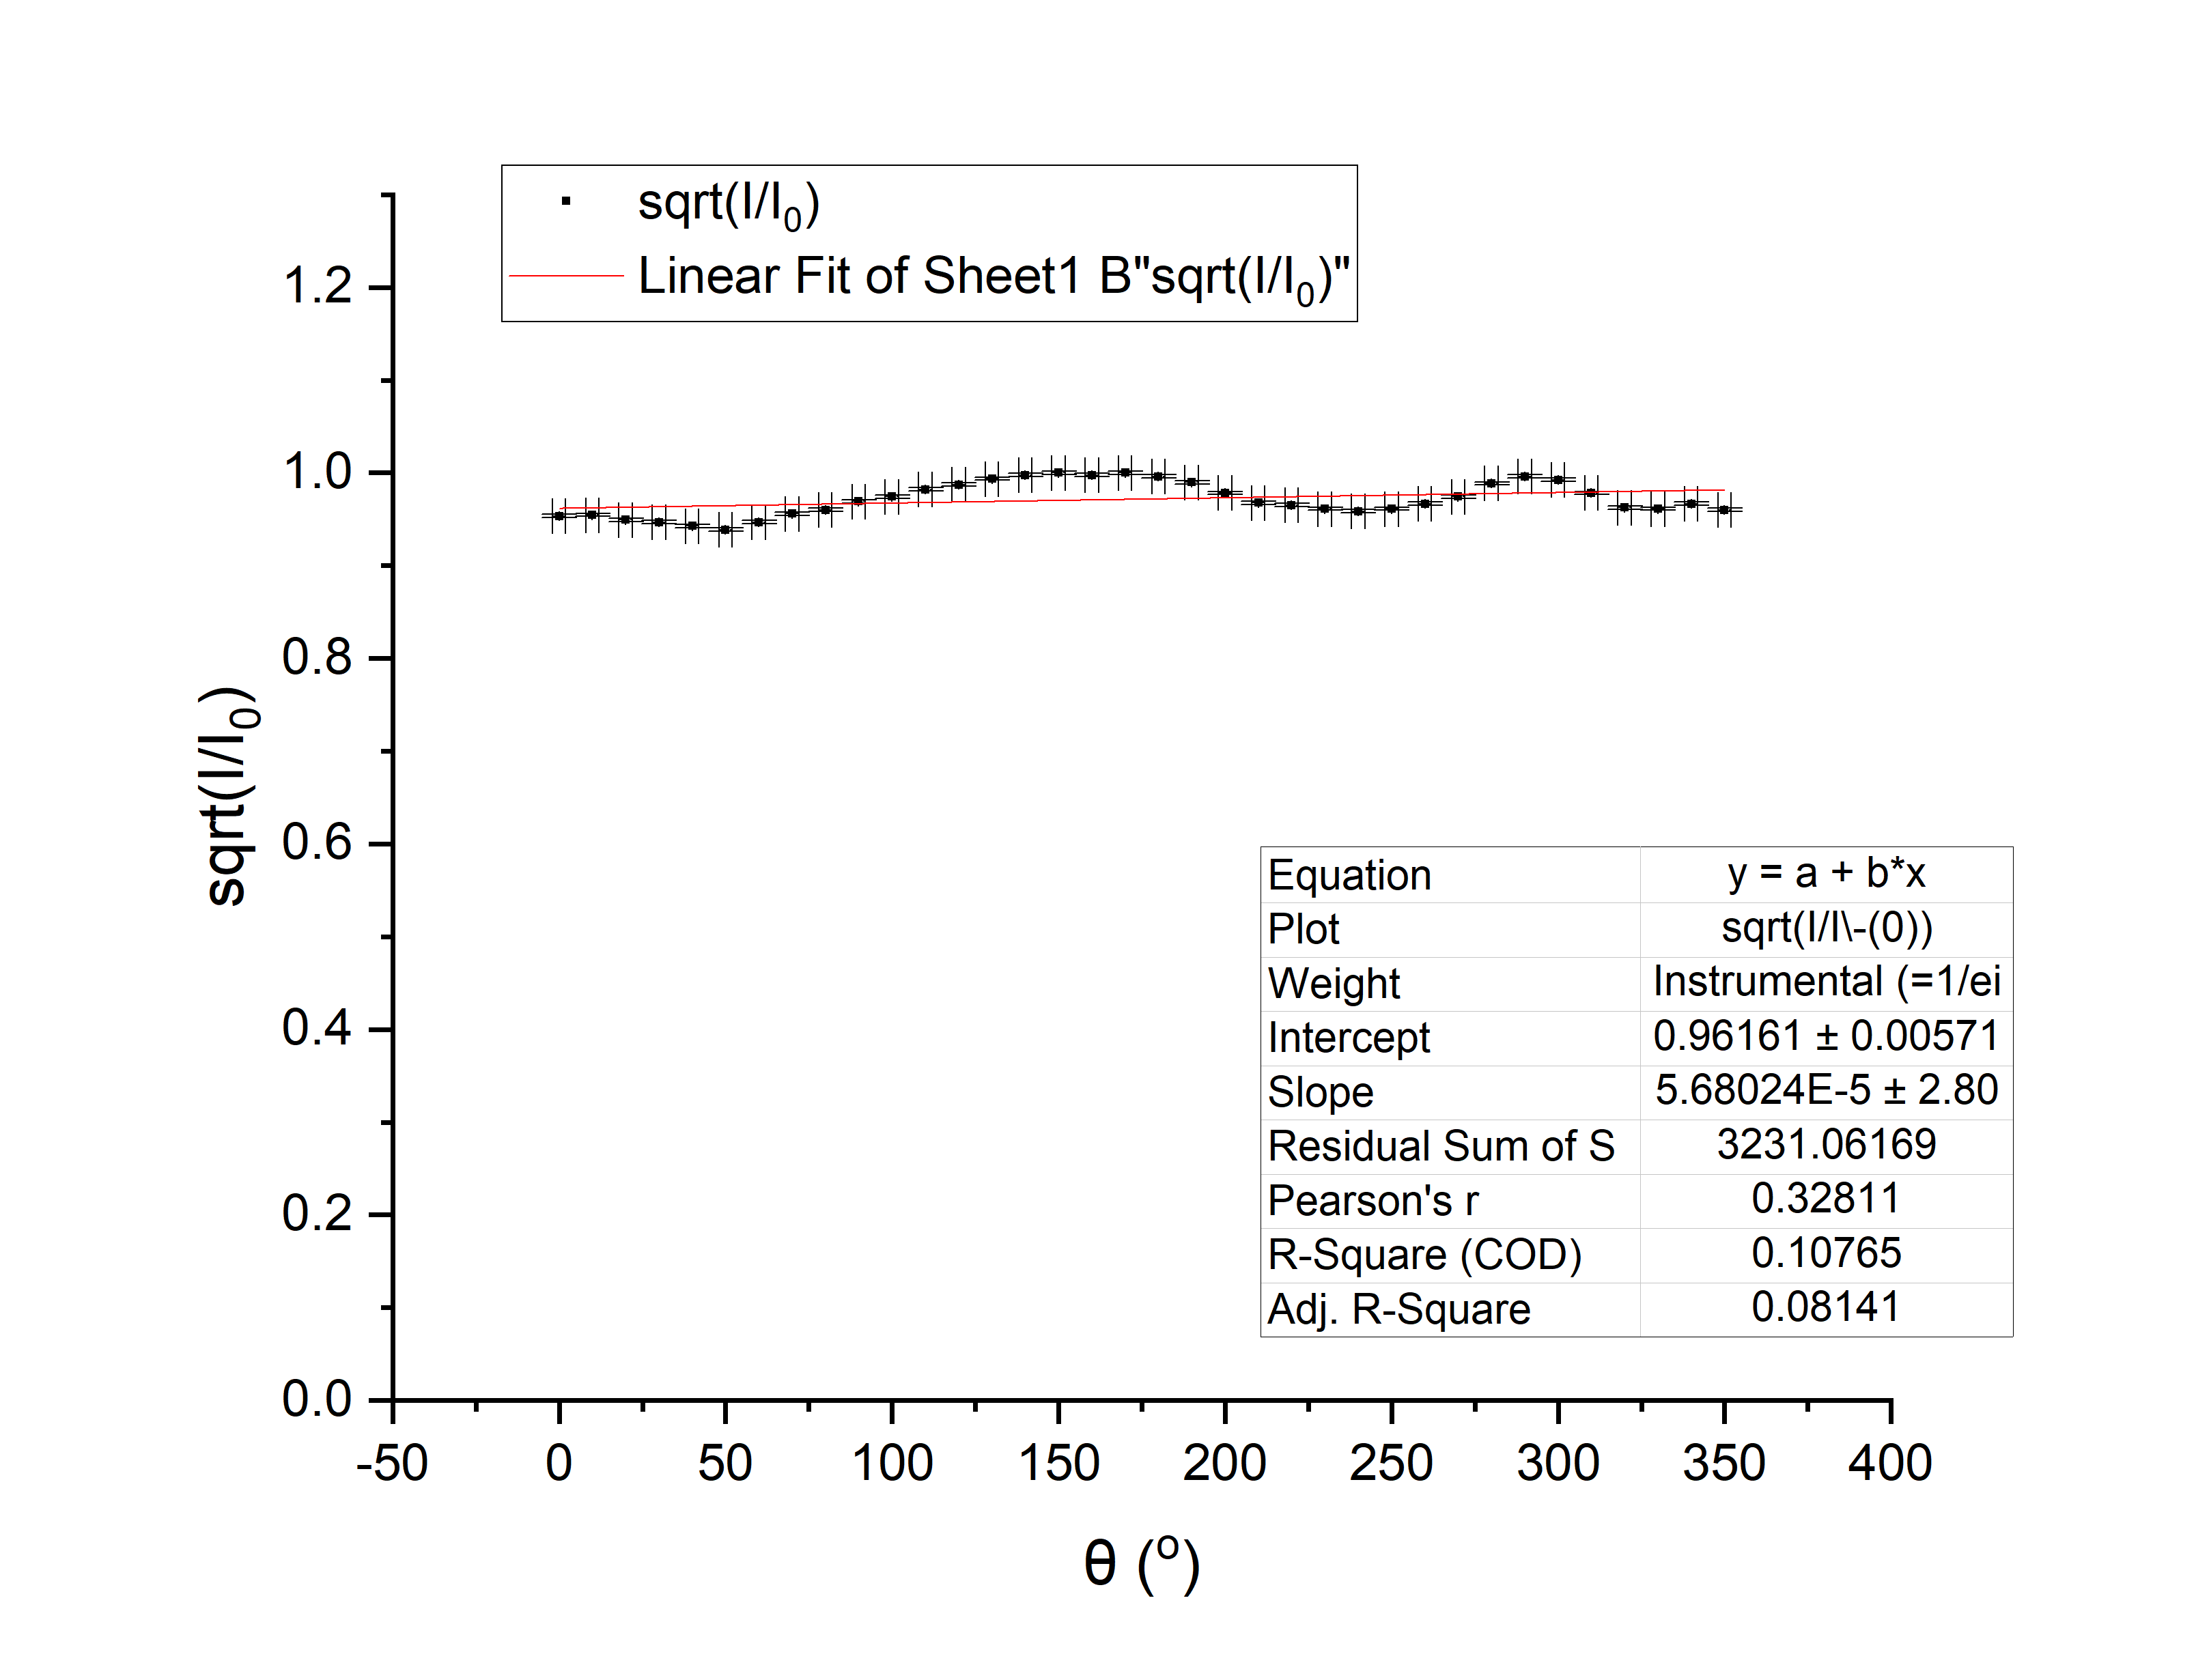
\includegraphics[scale=0.45]{6.png}
\caption{$\sqrt{I/I_0}$ vs. $\theta$ relation in the Cartesian coordinate.}\label{Fig45l}
\end{figure}

\subsubsection{Rotation Angle: 70$^\circ$}

In the condition of the rotation angle is 70$^\circ$, the data when the light intensity reaches its maximum are presented in Table \ref{Table70}. Still, the data is subtracted by 90$^\circ$. The position of this point is marked in red in Figure \ref{Fig20}. It can seen that the value of $\theta$ when the light intensity reaches maximum in the case of 70$^\circ$ rotation angle is nearly symmetric about $\theta = 0$ axis with that ($\theta = 20^\circ (200^\circ)$) in the case of 20$^\circ$ rotation angle. 

\begin{table}[H]\centering
\begin{tabular}{cc}
\toprule
\multicolumn{2}{c}{Rotation angle of the 1/4-wave plate: 70$^\circ$}\\
\midrule
$\theta\,\,[^\circ] \pm 2[^\circ]$ & 161 \\
$I\,\,[\mu\text{A}] \pm 0.001\,\,[\mu\text{A}]$ & 0.682 \\
\bottomrule
\end{tabular}
\caption{Measurement data for the 1/4-wave plate (rotation angle 70$^\circ$).}\label{Table70}
\end{table}

\section{Discussion and Conclusions}

\subsection{Demonstration of Malus' Law}

The slope of the fitting is 1.01 $\pm$ 0.02 and the Pearson's r is 0.99916, which is very close to 1. This suggests that the value of $I/I_0$ is proportional to the value of $\cos^2\theta$ with the coefficient to be about 1. Theoretically, by Eq. (\ref{eqMalus}), the slope is
$$\frac{I/I_0}{\cos^2\theta} = 1,$$
Therefore, the relative error is
$$\varepsilon = \frac{1.01-1}{1} \times 100\% = 1\%.$$
This in an acceptable range of error verifies the Malus' Law.

\subsection{Linearly Polarized Light and the Half-wave Plate}

The slope of the linear fit is $2.01 \pm 0.02$. Theoretically, as introduced in the Introduction part, the rotation angle of the polarization axis is twice of the origin angle for a half-wave plate. Therefore the theoretical value of the slope of our linear fitting is 2. The relative error is therefore
$$\varepsilon = \frac{2.01-2}{2}\times 100\% = 0.5\%.$$ 
This conforms to the theoretical fact.

\subsection{Circularly and Elliptically Polarized Light and the 1/4-wave Plate}

\subsubsection{Rotation Angle: 0$^\circ$}

From Table \ref{Table1/40} and Figure \ref{Fig0}, it can be seen that the 
maximum of light intensity occurs at about $\theta = 0^\circ$. This suggests that polarizing axis is parallel to the optical axis of the plate, which is the theoretical conclusion stated in the Introduction part. The shape of the plot also indicates that it is linearly polarized.

\subsubsection{Rotation Angle: 20$^\circ$}

From Table \ref{Table1/420} and Figure \ref{Fig20}, it can be seen that the 
maximum of light intensity occurs at about $\theta = 20^\circ$. This suggests that polarizing axis forms $20^\circ$ to the optical axis of the plate, which conforms to the fact stated in [2]. The shape of the plot also indicates that it is elliptically polarized.

\subsubsection{Rotation Angle: 45$^\circ$}

From Figure \ref{Fig45}, it can be seen that the value of $\sqrt{I/I_0}$ changes little when $\theta$ changes. Besides, the slop of linear fit of the plot of $\sqrt{I/I_0}$ vs. $\theta$ in the Cartesian coordinate in Figure \ref{Fig45l} is $6 \times 10^{-5} \pm 6 \times 10^{-5}$ and the Pearson's coefficient is only 0.328. All the results suggest that $\sqrt{I/I_0}$ is a constant, with no relation with the value of $\theta$. Therefore it can be concluded that when rotation angle is 45$^\circ$, the light is circularly polarized. This conforms to the fact stated in the Introduction part.

\subsubsection{Rotation Angle: 70$^\circ$}

From section 4.3.4, we can state that the value of $\theta$ when the light intensity reaches maximum in the case of 70$^\circ$ rotation angle is nearly symmetric about $\theta = 0$ axis with that ($\theta = 20^\circ (200^\circ)$) in the case of 20$^\circ$ rotation angle. This conclusion conforms to the theoretical conclusion stated in [2].

\subsection{Causes for errors and uncertainties}

Possible causes for errors and uncrtainties are listed below:

\begin{enumerate}
    \item The light of our torch may affect the light intensity detected by the photo-cell.
    \item The precision of the scale on the optical elements us $2^\circ$, which results in a relatively large uncertainty.
    \item It is really tough to adjust the center of all the optical elements to be in a line and we failed to do that in our experiment. This may lead to errors to the experiment.
\end{enumerate}

\subsection{Suggestions}

Some suggestions for further improvement:

\begin{enumerate}
    \item The experiment may be performed in an environment that is absolutely dark, where the readings are also available. 
    \item Improve the precision of the scale on the optical elements. 
\end{enumerate}

\subsection{Conclusions}
In this lab, we studied the polarization phenomenon and verify Malus' law. The way half- and quarter-wave plates work in optical systems is also explored. The experimental results we obtained is of relatively small uncertainties and conform to the theoretical facts in an acceptable range of uncertainty.

\begin{thebibliography}{1}

\bibitem{manual} VP241 Exercise 4: Polarization of Light, Department of Physics, Shanghai Jiaotong University.
\bibitem{textbook} University Physics, Section 33.5, Young and Freedman.

\end{thebibliography}

\newpage

\appendix

\section{Measurement Uncertainty Analysis}

\subsection{Uncertainty for Data in Demonstration of Malus' Law}

The uncertainty of $\cos^2\theta$ is 
\begin{align*}
u_{\cos^{2}\theta}&=\sqrt{(\frac{\partial \cos^{2}\theta}{\partial \theta}u_{\theta})^{2}}\\
&=|-2\cos\theta\sin\theta u_{\theta}|\\
&=|\sin2\theta u_{\theta}|,
\end{align*}
where $u_\theta = 2[^\circ] = \pi/90$. Take $\theta$ = 0 as an example, 
$$u_{\cos^{2}\theta}=|\sin2\theta u_{\theta}|=|\sin({2\times 5^\circ})\times \frac{\pi}{90}|=0.006,$$
All the results are shown in Table \ref{TableUncCI}.\\

The uncertainty of $I/I_0$ is 
\begin{align*}
u_{I/I_{0}}&=\sqrt{(\frac{\partial I/I_0}{\partial I}u_{I})^{2}+(\frac{\partial I/I_0}{\partial I_{0}}u_{I_{0}})^{2}}\\
&=\sqrt{(\frac{u_{I}}{I_{0}})^{2}+(-\frac{I}{I_{0}^{2}}u_{I_{0}})^{2}},
\end{align*}
where $u_I = u_{I_0} = 0.001\,\,[\mu\text{A}]$, $I_0 = 1.037 \pm 0.001\,\,[\mu\text{A}]$. Take the first set of data as an example,
$$u_{I/I_{0}}= \sqrt{(\frac{u_{I}}{I_{0}})^{2}+(-\frac{I}{I_{0}^{2}}u_{I_{0}})^{2}}=\sqrt{(\frac{0.001}{1.037})^{2}+(-\frac{1.037}{1.037^{2}}\times 0.001)^{2}}=0.0013,$$
All the results are shown in Table \ref{TableUncCI}.

\begin{table}[H]\centering
\begin{tabular}{cc||cc}
\toprule
$u_{\cos^2\theta}$ & $u_{I/I_0}$ & $u_{\cos^2\theta}$ & $u_{I/I_0}$\\
\midrule
    0     & 0.0013 & 0.03  & 0.0011 \\
    0.006 & 0.0013 & 0.03  & 0.0010 \\
    0.012 & 0.0013 & 0.03  & 0.0010 \\
    0.017 & 0.0013 & 0.03  & 0.0010 \\
    0.02  & 0.0013 & 0.02  & 0.0010 \\
    0.03  & 0.0013 & 0.017 & 0.0010 \\
    0.03  & 0.0012 & 0.012 & 0.0010 \\
    0.03  & 0.0012 & 0.006 & 0.0010 \\
    0.03  & 0.0011 & 0     & 0.0010 \\
    0.03  & 0.0011 &       &  \\
\bottomrule
\end{tabular}
\caption{Uncertainty of $\cos^2\theta$ and $I/I_0$.}\label{TableUncCI}
\end{table}

\subsection{Uncertainty for Linearly Polarized Light and the Half-wave Plate}

In this part, the uncertainty of the measurement depends on the device, which is 
$$u_\theta = 2^\circ.$$

\subsection{Uncertainty for Circularly and Elliptically Polarized Light and the 1/4-wave Plate}

The uncertainty of $\sqrt{I/I_0}$ is
\begin{align*}
u_{\sqrt{I/I_{0}}}&=\sqrt{(\frac{\partial\sqrt{I/I_0}}{\partial I}u_{I})^{2}+(\frac{\partial\sqrt{I/I_0}}{\partial I_{0}}u_{I_{0}})^{2}}\\
&=\sqrt{\frac{1}{4II_0}u_I^2+\frac{I}{4I_0^3}u_{I_0}^2},
\end{align*}
where $u_I = u_{I_0} = 0.001\,\,[\mu\text{A}]$, $I_0 = 0.805 \pm 0.001\,\,[\mu\text{A}]$ for rotation angle of 0$^\circ$, $I_0 = 0.707 \pm 0.001\,\,[\mu\text{A}]$ for rotation angle of 20$^\circ$, $I_0 = 0.395 \pm 0.001\,\,[\mu\text{A}]$ for rotation angle of 45$^\circ$. Take the first set of data as an example,
$$u_{\sqrt{I/I_{0}}}=\sqrt{\frac{1}{4\times 0.729 \times 0.805} \times 0.001^2+\frac{0.729}{4\times 0.805^3}\times 0.001^2}=0.0009.$$
All the results are shown in Table \ref{TableUnc1/4}.

\begin{table}[H]\centering
\begin{tabular}{ccc}
\toprule
Rotation angle: $0^\circ$ & Rotation angle: $20^\circ$ & Rotation angle: $45^\circ$\\
$u_{\sqrt{I/I_{0}}}$ & $u_{\sqrt{I/I_{0}}}$ & $u_{\sqrt{I/I_{0}}}$\\
\midrule
    0.0009  & 0.0010 & 0.0018 \\
    0.0009  & 0.0010 & 0.0018 \\
    0.0009  & 0.0010 & 0.0018 \\
    0.0009  & 0.0010 & 0.0018 \\
    0.0010  & 0.0010 & 0.0018 \\
    0.0011  & 0.0010 & 0.0018 \\
    0.0013  & 0.0010 & 0.0018 \\
    0.0018  & 0.0011 & 0.0018 \\
    0.003   & 0.0012 & 0.0018 \\
    0.010   & 0.0014 & 0.0018 \\
    0.004   & 0.0017 & 0.0018 \\
    0.0019  & 0.0019 & 0.0018 \\
    0.0013  & 0.0018 & 0.0018 \\
    0.0011  & 0.0015 & 0.0018 \\
    0.0009  & 0.0013 & 0.0018 \\
    0.0009  & 0.0011 & 0.0018 \\
    0.0009  & 0.0011 & 0.0018 \\
    0.0009  & 0.0010 & 0.0018 \\
    0.0009  & 0.0010 & 0.0018 \\
    0.0009  & 0.0010 & 0.0018 \\
    0.0009  & 0.0010 & 0.0018 \\
    0.0009  & 0.0010 & 0.0018 \\
    0.0009  & 0.0010 & 0.0018 \\
    0.0010  & 0.0010 & 0.0018 \\
    0.0013  & 0.0010 & 0.0018 \\
    0.0018  & 0.0011 & 0.0018 \\
    0.003   & 0.0012 & 0.0018 \\
    0.010   & 0.0014 & 0.0018 \\
    0.004   & 0.0017 & 0.0018 \\
    0.0019  & 0.0019 & 0.0018 \\
    0.0013  & 0.0018 & 0.0018 \\
    0.0011  & 0.0015 & 0.0018 \\
    0.0010  & 0.0013 & 0.0018 \\
    0.0009  & 0.0012 & 0.0018 \\
    0.0009  & 0.0011 & 0.0018 \\
    0.0009  & 0.0010 & 0.0018 \\
\bottomrule
\end{tabular}
\caption{Uncertainty for $\sqrt{I/I_0}$ when the rotation angle is $0^\circ$, $20^\circ$ and $45^\circ$.}\label{TableUnc1/4}
\end{table}

\section{Data Sheet}

Please find the original data sheet attached at the end of the report.

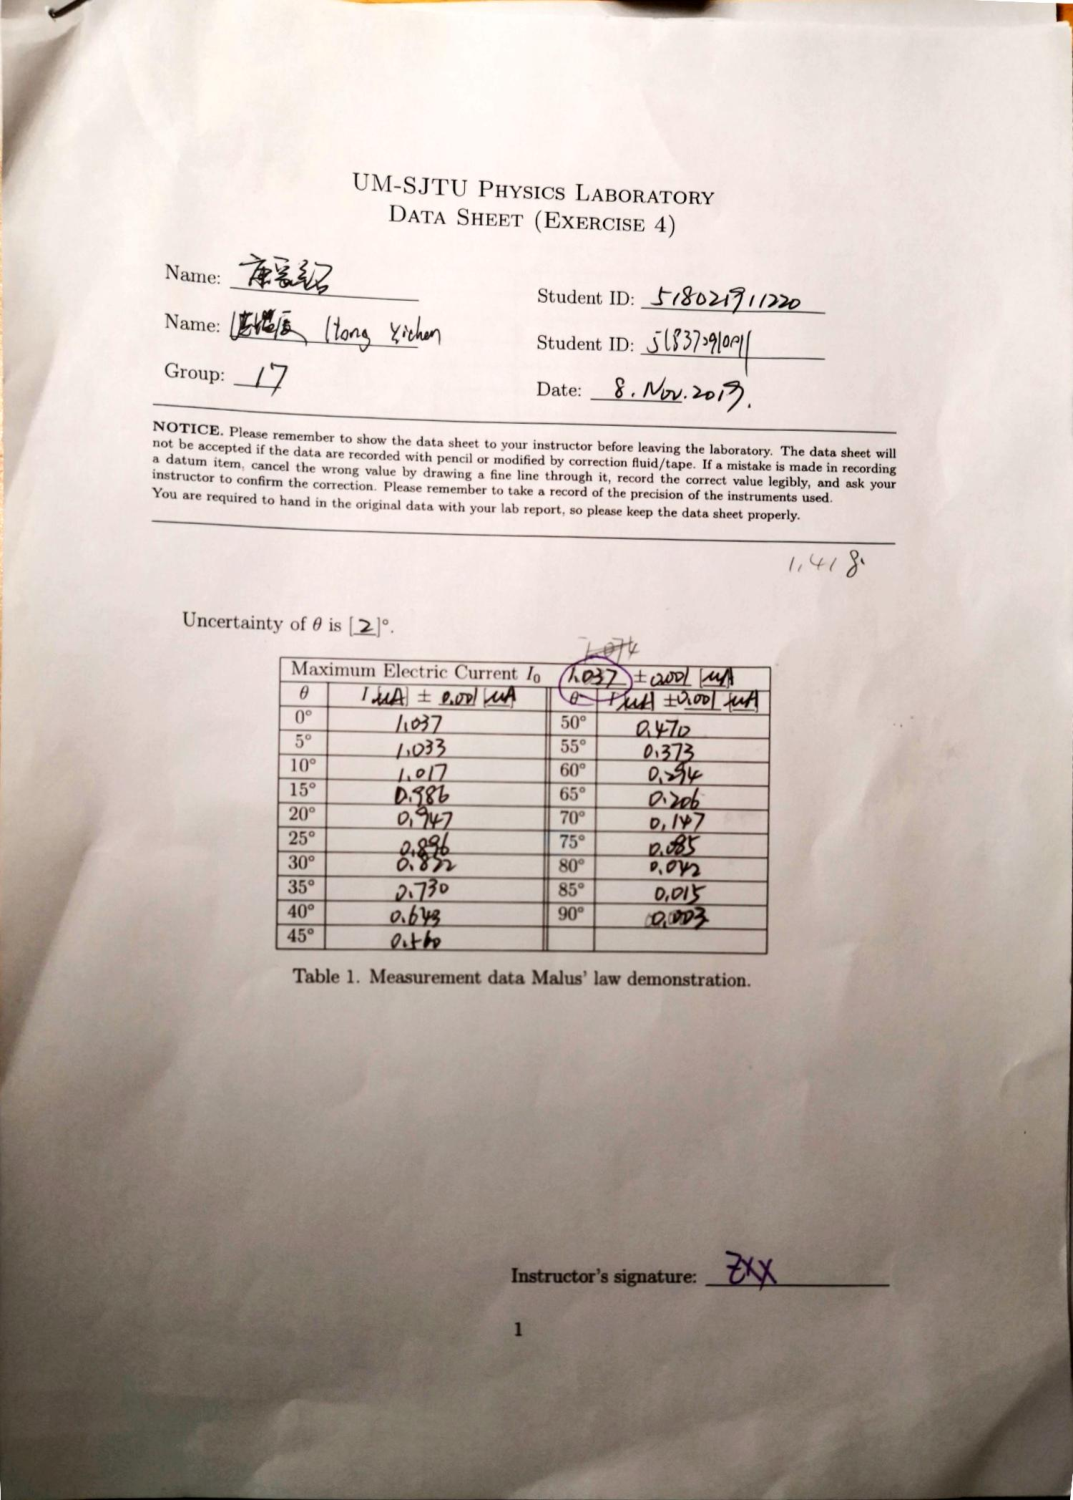
\includepdf[pages=-]{lab4datasheet.pdf}

\end{document}
